\chapter{Efficient Learning and Unlearning via Large-Scale Conditional Independence Testing} \label{chap:lcodec} 
\todo{ch5 notation pass, remove redundant bknd}

While selecting a more efficient model \textit{a priori}
can be helpful when we can plan ahead of training,
it may sometimes be the case
that a task may require selection
after a model has been trained.
In this chapter we will 
address this post-hoc selection task
from a parameter-focused point of view,
motivated by the need for an efficient way of 
``scrubbing'' existing models of samples
they have been trained on.
At this time, unlearning in this context has
only been analyzed under the assumption
that model updates can be made over the \textit{entire} model, but the forms of provable updates have limited
practical deployments for feasibility
as we will see.
Using conditional independence ideas
we will identify a parameter subset sufficient for
efficient unlearning.
Work in this chapter was first published
in the conference on Computer Vision and Pattern Recognition~\citep{lcodecunlearn}.

\section{Introduction}
The use of Optimal transport (OT) is now prevalent in many problem settings including information retrieval \citep{balikas2018cross,yurochkin2019hierarchical}, image processing \citep{otip}, statistical machine learning, as well as more recently, for ethics and fairness research \citep{kwegyiraggrey2021relative}. 
OT is well-suited for tasks where dissimilarity between two or more probability distributions must be quantified; 
its success was made possible through dramatic improvements in algorithms \citep{cuturi2013sinkhorn,solomon2015convolutional} that allow one to efficiently optimize commonly used functionals.
In practice, OT is often used to estimate and minimize the 
distance between certain (data-derived) distributions, 
using an appropriately defined loss functional. %Recent advances provide us the capability to drop-in and seamlessly integrate many types of losses into existing methods, for novel applications.
When one seeks to operate on more than two distributions, however, newer constructions are necessary to effectively estimate distances and transports.
To this end, a well studied idea in the literature is the ``barycenter,''
identified by minimizing the pairwise distance between itself and all other distributions given. 
The $d$-dimensional proxy distance is then defined as the sum of the distances to the barycenter.

%\begin{comment}
%\vikas{the following paragraph is low on content. Perhaps take 1-2 initial lines, compress and use it close off the previous paragraph?}
%The driving practical focus of optimal transport aims to estimate and minimize the distance between distributions of interest. Within machine learning, this takes the form of a loss; recent developments have enabled constructions of such a loss that allow almost seamless integration into existing methods. These incorporations have led to a number of benefits over traditional mean-squared error approaches, taking direct advantage of the statistical and distributional assumptions and requirements of the model fitter.
%\end{comment}

% {\bf Barycenters.} 
%While distances are defined between two points (or two probability distributions), barycenters extend the idea and enable analyzing many points (or probability 
% One way to quantify dissimilarity between many distributions is through distance to the mean. Here, for averaging,  
% we measure pairwise distances.
% Practically, this has led to models that can 
% concurrently enforce distributional similarity between a 
% set of distributions and has found use in 
% a spectrum of applications, which we will list shortly.

{\bf Computing barycenters.} 
Assuming that a suitably regularized form of the optimal transport loss is utilized, the pairwise distance 
calculation, by itself, can be efficient -- in fact, 
in some cases, Sinkhorn iterations can be used \citep{cuturi2013sinkhorn}. 
On the other hand, to minimize distances to the mean, 
most algorithms typically operate 
by repeatedly estimating the barycenter and those pairwise distances, and using a ``coupling'' strategy 
to push points toward the barycenter,
or in other cases, summing over all pairwise 
distances. 
% \glenn{I wonder if our method could be also more robust when the pairwise distances are very non-uniform, especially at early iterations...see  \href{https://www.stat.cmu.edu/~larry/=sml/Opt.pdf}  {https://www.stat.cmu.edu/~larry/=sml/Opt.pdf}at the end of page 10}\ronak{I like this idea, maybe we can allude to it briefly?}
%The idea is sensible but a
As the number of distributions 
grows, robustness issues can exacerbate \citep{alvarez2008trimmed} and the procedure is 
expensive (e.g., for 50 distributions, 50 bins).
%{\color{red}For example, even on a high end workstation, 
%simply computing the barycenter over
%50 distributions with 50 bins}
%does not converge within a reasonable number of iterations
%using newer packaged solvers. {\color{red} maybe instead of ``not...reasonable'', try ``not competitive"}
%is a time-intensive process.

% {\bf An efficient alternative.}
{\bf A potential alternative.}
Multi-marginal optimal transport (MMOT) is a related problem to the aforementioned task but to some extent, the literature has developed in parallel.
In particular, MMOT focuses on identifying a joint distribution such that the marginals are defined by the input distributions over which we wish to measure the dissimilarity.
The definition naturally extends the two-dimensional formulation, and recent work has explored a number of applications \citep{pass2015multi}.
But the MMOT computation can be quite difficult,
and only very recently have practical algorithms been identified \citep{mmotcuturi}.
Additionally, even if a suitable method for computing an analogous measure of distance were available, 
\textit{minimizing} this distance to reduce 
dissimilarity (push distributions closer to each other) is practically hard if standard interior point solvers are needed just to compute the distance itself.
% however very recent research has shown that there exist polynomial time algorithms for this problem 
%have been shown to exist within the last year
% \cite{altschuler2021wasserstein}. Multimarginal versions of optimal transport have been studied but only few have led to practical algorithms \cite{mmotcuturi}.
% \vikas{can we concretize it 
% a little more? cite some numbers on a standard workstation? memory requirements? other resource needs?}
 %{\color{red} Glenn: fairness lead}

% {\color{red}this para does not add much}
% Importantly, we should also appreciate that the calculation of the barycenter is often a means to an end in most learning applications -- 
% the ultimate goal tends to be pushing these distributions to come closer. 
% A barycenter is a modeling choice, but other options may also be viable. 
% Indeed, if a different global measure of ``distributional disparity''
% were to be defined and minimized, the costs associated with pairwise comparisons and optimization
% may potentially be avoided. This hypothesis drives much of our development.

% \vikas{We need some work to justify the role/need of the following paragraph. What is the information is is designed to convey?} \glenn{I think we need to enforce this paragraph by contrasting it with our proposed approach, which I think its the intention of providing this information}
\noindent\textbf{Why and where is dissimilarity important?}
% {\color{red} START} Putting aside the cost to compute the barycenter for the moment, 
% instantiations of such applications often desire to enforce distribution similarity
% only on model outputs.
% For example, in \cite{jiang2020wasserstein}, the authors define fairness measures over the probability of the prediction given ground truth labels.  
% This choice is not without good reasons: discrete outputs lead to extremely nice distributions over the probability simplex, where optimization is easy and assumptions need not be strong.{\color{red} END; could START--END be replaced with the gray text?}
Enforcing distributions to be similar is a generic goal whenever one wishes some outcome of interest to be agnostic about particular groups within the input data.
In applications where training deep neural network models is needed,
% In applications,
it is often a goal to enforce distribution similarity on model outputs. 
For example, in \cite{jiang2020wasserstein}, the authors define fairness measures over the probability of the prediction, given ground truth labels.   
%FIXME: if you read this and know what X Y and Z are, then fill in and uncomment. This leads to distributions over the probability simplex with the desirable qualities X, Y and Z.
% 
However, these methods are rarely extended to continuous measures 
among internal neural network activations,
%(e.g., Bayesian networks), 
mainly due to the strong distributional assumptions needed (product of Gaussians) and the added algorithmic complexity of estimating the barycenter.
These issues limit application of these ideas 
%assumption-free distribution enforcement 
to only the final outputs of neural network models, where the distribution is typically binomial or multinomial.
% One drawback of this choice means that the distributional closeness is only guaranteed over the global model output {\vikas: this is unclear}, and little can be said about layer outputs prior to the thresholding for prediction.
MMOT solutions might be employed here, but suffer similar computational limitations.
% Additionally, full retraining would be necessary if thresholds must be adjusted due to changing business or regulatory requirements.

\noindent\textbf{Contributions.}  \textbf{(1)} We identify a particular form of the discrete multi-marginal optimal transport problem
which admits an extremely fast and numerically robust solution.
Exploiting a recent extension of 
the classical Earth Movers Distance (EMD) to a higher-dimensional Earth Mover's objective,
we show that such a construction is equivalent
to the discrete MMOT problem with Monge costs.
\textbf{(2)} We show that minimization of this \textit{global} distributional measure
leads to the 
harmonization of input distributions very similar in spirit to the minimization of distributions to barycenters (see Figure~\ref{fig:hists}).
\textbf{(3)} We prove theoretical properties of our scheme, and show that 
the gradient can be read directly off from a primal/dual algorithm,
alleviating the need for 
computationally intense 
pairwise couplings needed for barycenter approaches.
\textbf{(4)} The direct availability of the gradient
enables a specific neural network instantiation,
and
with a particular scaffolding provided by differentiable histograms, 
we can operate directly on network activations (anywhere in the network) to compute/minimize the d-MMOT. 
%The proposal integrates nicely with 
%existing pipelines. 
We establish via experiments that computing gradients used in backpropagation is fast, due to rapid access to solutions of the dual linear program.
We compare with barycenter-like approaches in several settings, including common fairness applications.
%, and show that our proposal 
%Our final construction,
%the $d$-dimensional Earth Mover's Distance (DEMD),
%integrates nicely with existing neural network pipelines. 

\begin{figure}[t]
    \centering
    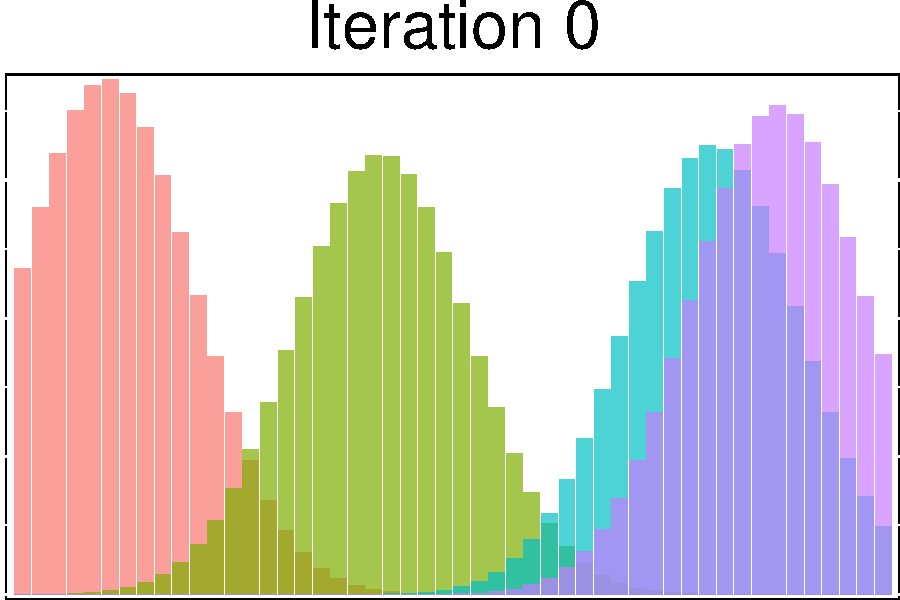
\includegraphics[width=0.19\textwidth]{6_demd/figs/hists/hists_iter_0.pdf}
    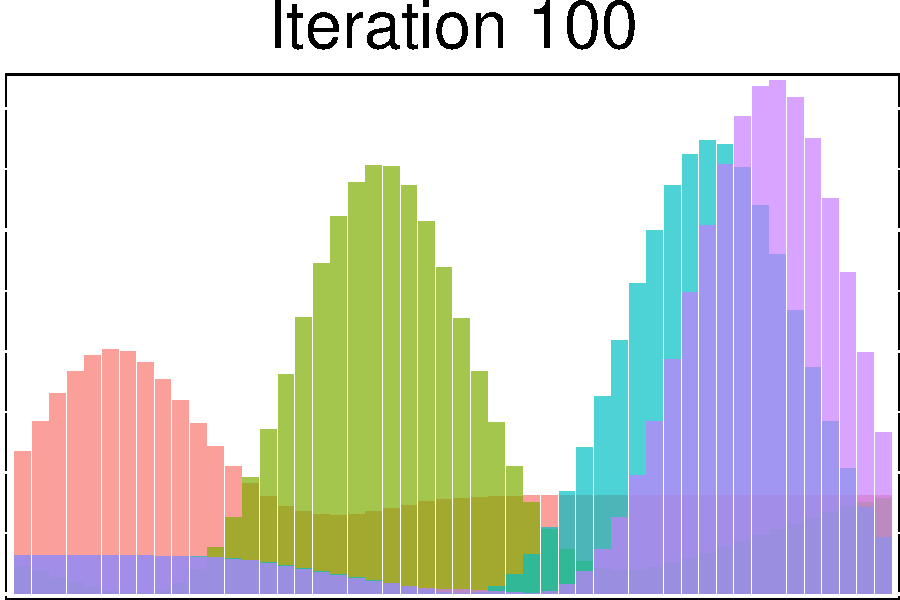
\includegraphics[width=0.19\textwidth]{6_demd/figs/hists/hists_iter_100.pdf}
    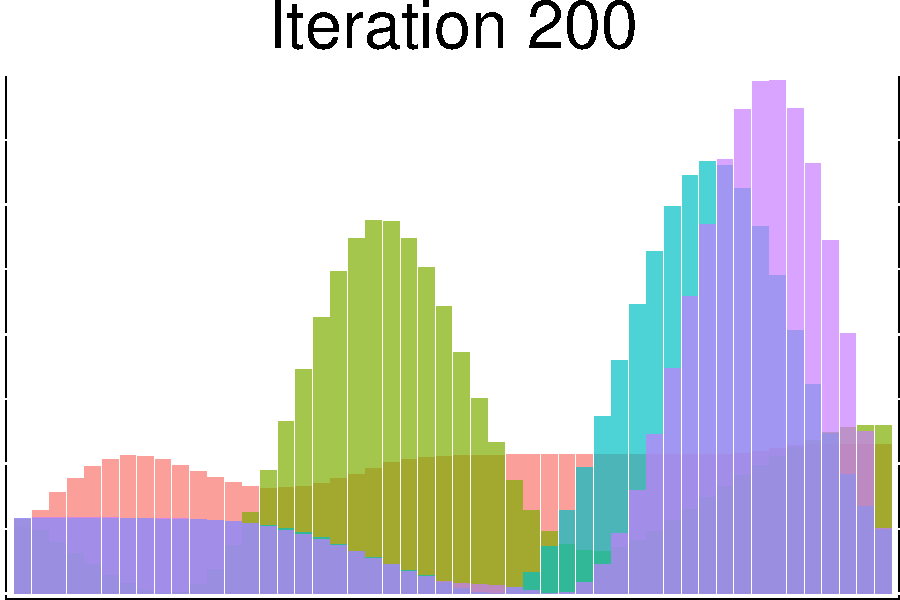
\includegraphics[width=0.19\textwidth]{6_demd/figs/hists/hists_iter_200.pdf}
    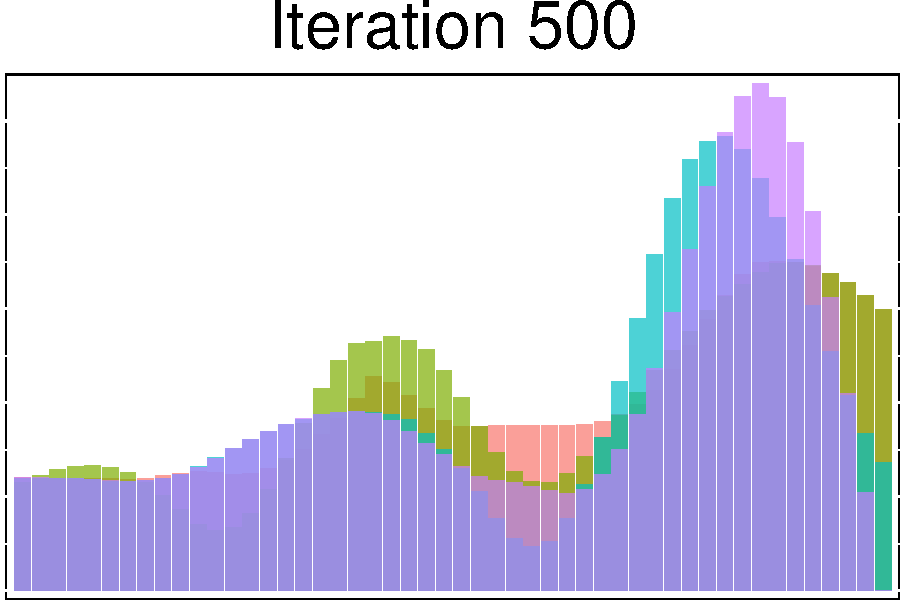
\includegraphics[width=0.19\textwidth]{6_demd/figs/hists/hists_iter_500.pdf}
    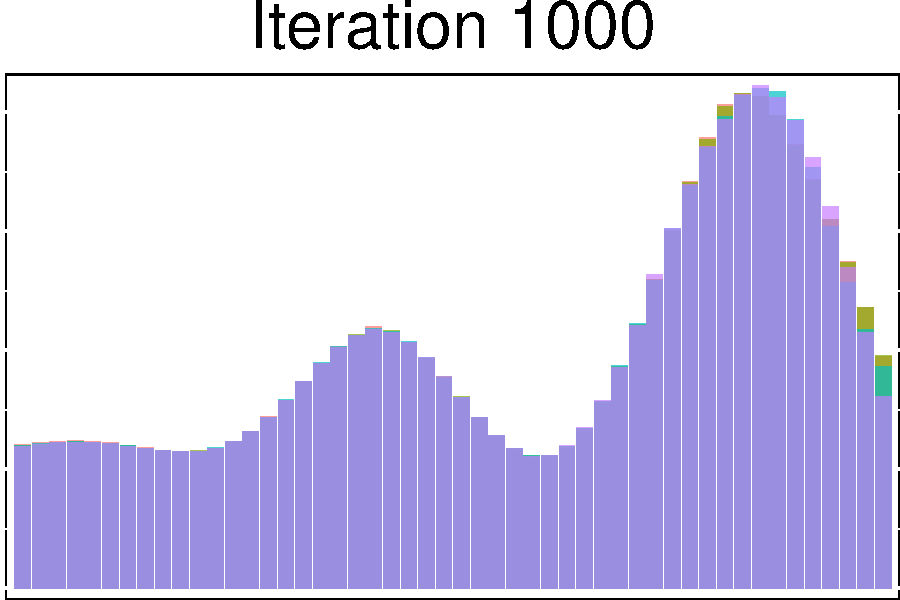
\includegraphics[width=0.19\textwidth]{6_demd/figs/hists/hists_iter_1000.pdf}
    \caption{\footnotesize Starting and ending state of minimizing a multi-marginal OT distance. Each iteration minimizes the generalized Earth Mover's objective, and then updates each histogram in the direction provided by the gradient.}
    \label{fig:hists}
    \vspace{-10pt}
\end{figure}

%%%% OLD
% In this work, we identify a simple {\em global} distributional measure with scaffolding that allows for fast computation over any continuous model output. A new multi-dimensional generalization of the classical Earth Mover's distance has recently been shown to be efficiently computable, and further developments show  that its minimization is extremely fast compared to existing barycenter-style methods.
% Functionally, it
% possesses several useful ingredients: (a) it requires no distributional assumptions, (b) it is efficient to compute, (c) its gradient is also efficiently computable. As a result, the functional can be 
% directly used in regimes where gradients are required for optimization (e.g., backpropogation and other gradient descent methods). 
% Finally, the functional is  numerically stable, and has an intuitive interpretation which facilitates interpretative reasoning.  
% In this work, we identify a simple {\em global} distributional measure with scaffolding that allows for fast computation over any continuous model output. A new multi-dimensional generalization of the classical Earth Mover's distance has recently been shown to be efficiently computable, and further developments show  that its minimization is extremely fast compared to existing barycenter-style methods. Functionally, it
% %distributions are computed over the invariant sets, a barycenter is computed as for the measure of invariance, and heuristic methods are employed to reducing the measured invariance in the loop. 
% Although these approaches aim to directly address the heterogeneity in the model output, they require (1) particular algorithms and solvers for relaxing discrete outputs to enable backpropogation and (2) that operating points and thresholds determining the final prediction are fixed. 
% If a method to operate directly on the activations prior to thresholding was feasible...
% Operating directly on the activations has its own hurdles.
% The activations are continuous, and so distributional assumptions must be made if any computation in the learning pipeline is to remain tractable. However a priori these assumptions are explicitly unknown. 
% \vikas{this appears to be tailored to the above paragraph. Ideally, we should start by highlighting a feature that allows moving away from the pairwise iterative scheme of barycenters.}
% In this work, we observe that a \textit{discretization} of continuous layer outputs allows for the computation of a new multi-distributional generalization of the classical Earth Mover's Distance (EMD) that allows for drop-in computation of disparity at the activation-level. 
% A common application of optimal transport incorporates the concept into a machine learning model by appending a suitable regularization term to the model's objective function.  Typically, this regularization term has the effect of making the statistical distribution of subsets of solutions either more uniform or else invariant in some prescribed way.  An illustration of a prototypical process appears in Figure~\ref{fig:hists}.
% In this paper, we apply a multi-distributional generalization of the classical Earth Mover's distance to the task of regularizing network models.
% The generalization that we employ is based on the classical Earth Mover's Distance (EMD), and
% We demonstrate that this functionally 
% possesses several useful ingredients: (a) it requires no distributional assumptions, (b) it is efficient to compute, (c) its gradient is also efficiently computable. As a result, the functional can be 
% directly used in regimes where gradients are required for optimization (e.g., backpropogation and other gradient descent methods). 
% Finally, the functional is  numerically stable, 
% and has an intuitive interpretation which facilitates interpretative reasoning.  
% Empirical demonstrations of the speed and viability of our approach are presented in Section~\ref{sec:results}.
% We take direct advantage of linear programming formulations of the EMD in its generalized form, and show that in fact the gradient can be directly identified as the solution to the dual program. Recent algorithmic developments allow for the primal and dual to be solved concurrently, allowing for a no-cost gradient computation if the forward computation is chosen accordingly.
% Whereas the classical Earth Mover's distance defines a distance metric between pairs of distributions, the generalized Earth Mover's objective defines a natural way to  measure  dissimilarity amongst $d\geq 2$ distributions. 
% Both the classical distance and the generalized objective can be expressed as linear programs.
% One advantage of the linear program formulation is the fact that every linear program has an equivalent {dual} linear program.
% We demonstrate, using standard sensitivity analysis, that solutions to the dual linear program equal the primal objective functional's gradient. If the functional is regularizing a neural network model, this gradient can be used for backpropagation of derivatives during model training.
% Additionally, it was recently shown that solving both the primal and dual linear programs of the generalized Earth Mover's objective can be accomplished in linear time and constant space by applying a straightforward  greedy algorithm. In experiments, we compare the speed to compute the gradients of the generalized Earth Mover's objective of the greedy algorithm against native auto-gradient procedures, and we demonstrate over $1000$-fold speed improvement. The method we describe is numerically stable, as no division operations or unusually large quantities are invoked in the process of solving the linear programs.  
% In many settings, however, a strict set of assumptions is required to apply and compute these existing methods. Particularly, optimal transport measures over continuous spaces are only practical when strong distributional assumptions can be made, and while discrete assumptions allow for more broad computation, they tend to poorly capture and generalize the actual measures of interest.
% An important feature of our approach is that it acts on model outputs prior to thresholding, so invariances to be maintained across varying thresholds.
% Our procedure addresses both of these limitations directly, by first promoting invariance at all discretizations of model outputs \textit{prior to thresholding}, and by making use of a differentiable histogramming procedure to directly apply precomputed gradients through backpropagation.
% A challenge in practical implementations that use this architecture  define invariance can be based on business or regulatory constraints, but these constraints can change over time.  Industry deployments of ML pipelines are not compatible with such a setting is an important way: thresholds considered for discretization or classification are often adjusted or changed due to changing business or regulatory directives.   After training with procedures similar to the above, no guarantee regarding invariance can be made if the threshold is changed. It is often not sufficient or even feasible to retrain when operating points may or must change.
% {\color{red} redundant, merge with above para}
% \noindent\textbf{Contributions.} In this work, we present an application of a recent extension of the classical Earth Movers distance to a higher-dimensional Earth Mover's objective.
% We show that minimization of the objective leads to the harmonizing (lang) of input distributions similar to the minimization of distributions to barycenters.
% We prove theoretical properties of the objective and the procedure that
% reveals the gradient can be read directly off from a primal/dual algorithm,
% alleviating the need for computing intensive pairwise couplings.
% % This objective provides an alternative to barycenter approaches as a way to regularize network models in a way that reduces statistical dissimilarity of the optimal solutions. % The functional we use acts on a \textit{discretized version} of model outputs prior to thresholding, and allows for invariances to be maintained across varying thresholds. 
% With a particular instantiation of differentiable histograms, we can apply and smoothly operate directly on network activations to compute the EMD measure. 
% We establish through experiment that the speed of computing gradients used in backpropogation can be computed in substantially shorter times than one can achieve using standard tools, due to rapid access to solutions of the the dual linear program formulation.
% We compare and contrast the performance and speed of our construction against Barycenter-like measures in a number of settings and demonstrate applications in a common fairness setting.
% Our final construction integrates seamlessly with existing neural network pipelines.
% Machine learning has become ubiquitous, but has suffered some setbacks in public and regulatory visions due to issues typically considered orthogonal to traditional measures of success within the literature.
% Most modern advancements in machine learning follow from learning a model that optimizes for some measure of \textit{accuracy}, measured by misclassification errors over all samples or global measures of true and false positive and negative rates.
% Unfortunately, when statistical assumptions of homogeneous data fail, these measures can be skewed heavily towards subsets of the data that follow a majority or the primary mode of the underlying distribution. These biases can take many forms, and in applications in which data and outcomes may be represent people and decisions for those people, can lead directly towards unfairness and disparity among groups.
% The last few years of machine learning deployment has revealed a myriad of situations in which strong bias and fairness concerns have led to strong social backlash. Examples: COMPAS, twitter, etc. \cite{?}
% With these concerns has also come interest in technical solutions to fairness and bias. Several conferences and workshops have been created \cite{fat, facct, etc}, devoted to grounding and understanding these ideas within a mathematical and statistical context. From these communities concrete definitions have been formed, along with a number of algorithmic solutions to both avoid and account for bias and unfairness within both data and models.
% Existing methods for accounting for fairness typically define measures over discrete output spaces, and attempt to minimize some measure of disparity between these discrete probabilities. Varying definitions of fairness have been constructed under this umbrella, and a number of nice solutions have been proposed that allow for fair regularization in traditional machine learning training pipelines.
% A drawback to these approaches is that they rely on the discrete/binary outputs of models to be fixed: once a model is trained, the threshold used for those outputs cannot be changed else all fairness guarantees provided by the regularization fail, because the output distributions have all been constructed with that specific threshold. Practical deployments of machine learning models in industry rely on being able to select different points of operation, to match secondary requirements or measures provided by business or regulatory requirements. In these cases it is not sufficient or feasible, especially for large models, to create and retrain methods when these operating points must change. Their is a clear need for methods which are fair across potentially many points of operation.
% While moving to fairness over the continuous measure prior to thresholding may be infeasible, new results suggest that discretization at points of operation can lead to practical solutions for constructing models fair over many thresholds.
% \noindent\textbf{Contributions.} In this work, we analyze fairness from a new perspective. By looking at the distances between distributions over discretized spaces prior to thresholding for downstream discrete tasks, we apply a recently developed tool for computing EMD distance to quickly measure the disparity between groups over discretized continuous measures. Using a key observation that the gradients are readily available, we directly incorporate this EMD distance into standard machine learning pipelines. 
\begin{figure}
    \centering
    % 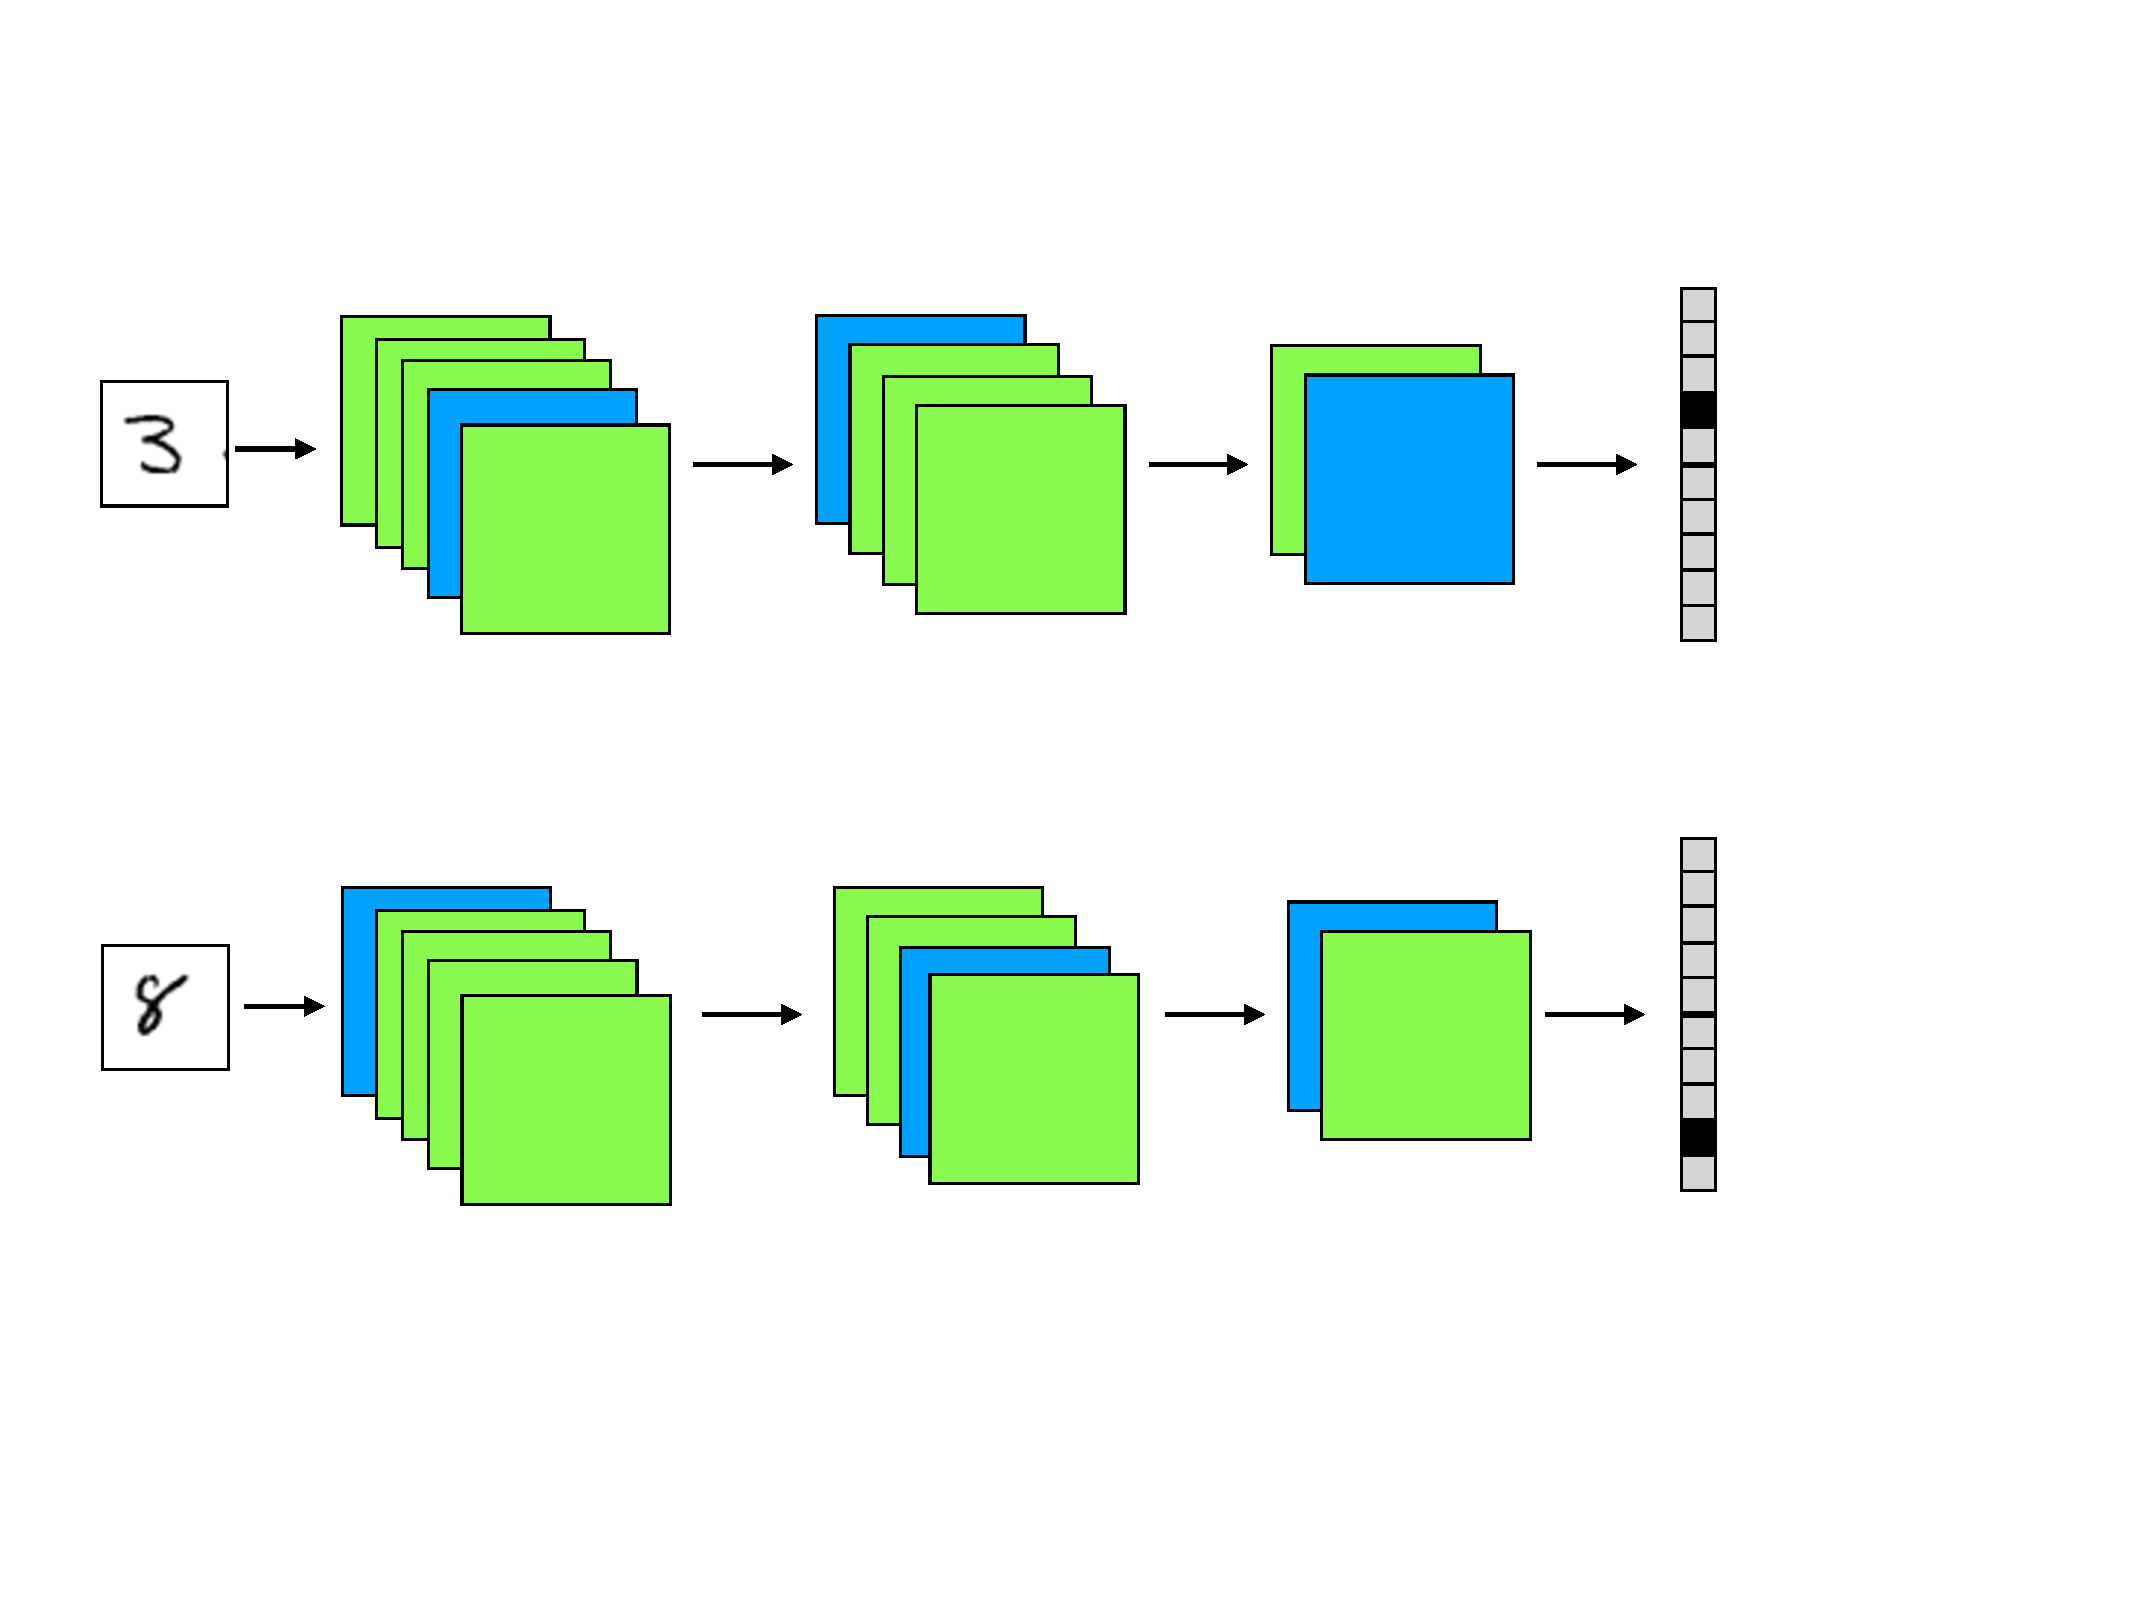
\includegraphics[height=1.5in,trim={1.5cm 5cm 3cm 3.5cm},clip]{figs/layercnn.pdf}
    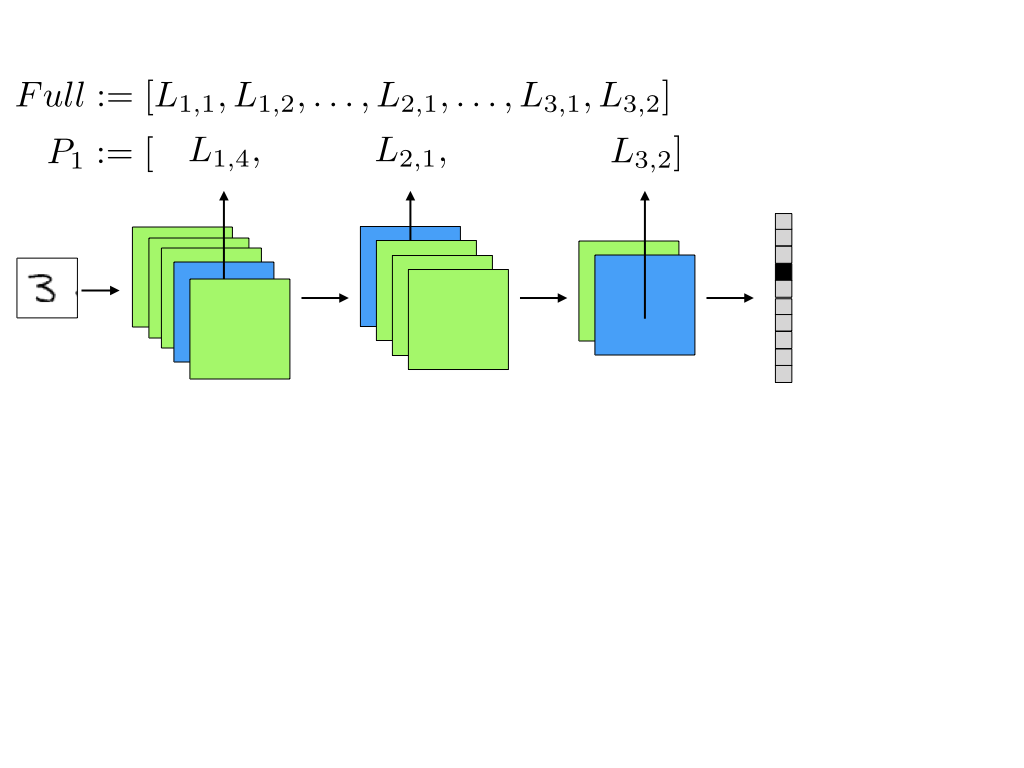
\includegraphics[width=\columnwidth,trim={0cm 12cm 5cm 2.5cm},clip]{5_unlearn/figs/layercnn.png}
    \caption[Conditionally independent network subsets]{\label{fig:main1} Large deep learning networks typically associate specific subsets of network parameters, blocks (blue), to specific samples in the input space.
    Traditional forward or backward passes may not reveal these blocks: high correlations among features may not distinguish important ones. Input perturbations can be used to identify them in a probabilistic, distribution-free manner.}
\end{figure}
\begin{figure}
	\centering
	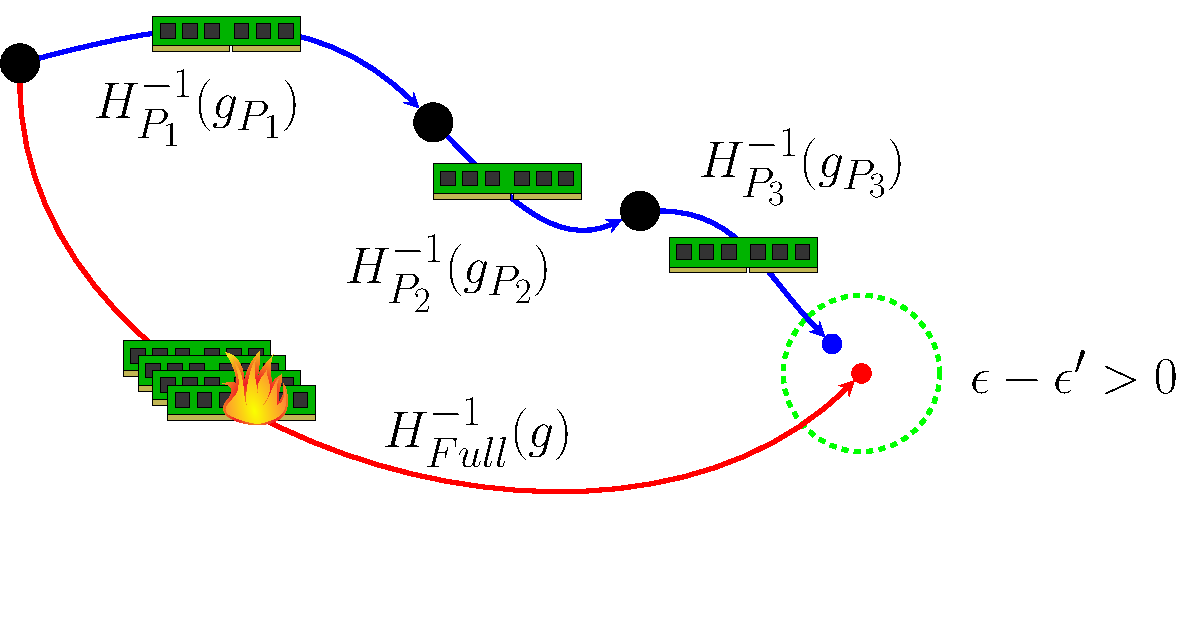
\includegraphics[width=\columnwidth,trim={0cm 1cm 0cm 0cm},clip]{5_unlearn/figs/unlearning_fig.pdf}
	\caption[Efficient unlearning]{\label{fig:main2}Network blocks can be unlearned together in an efficient block-coordinate style update (blue lines), approximating an update to the full network which requires a costly, and sometimes infeasible due to memory constraints, full Hessian inverse (red line).}
\end{figure}

\section{Problem Setup for Unlearning}
Let $\cA$ be an algorithm that takes as input a training set $\cS$ and outputs a hypothesis $w \in \cW$, defined by a set of $d$ parameters $\Theta$. 
An unlearning scheme $\cU$ takes as input a sample $z' \in \cS$ used as input to $\cA$, and ideally, outputs an \textbf{updated} hypothesis $w' \in \cW$ where $z'$ has been deleted from the model.
%
% Clearly within unlearning we do not wish to simply rerun $\cA$ on the subset without the sample to delete.
% Particularly for modern machine learning problems with extremely large datasets and model architectures, retraining can be costly or impossible.
%
% Retraining may be costly or impossible, but provides a baseline oracle to which we can compare updates as in \eqref{eq:unlearn}.
% However, this provides a baseline with which we can compare any other potential unlearning algorithm to.
% Namely, a
An unlearning algorithm should output a hypothesis that is close or equivalent to one that would have been learned had the input to $\cA$ been $\cS \setminus z^\prime$. A framework for this goal was given by \cite{ginart2019making} as,
% Following \cite{sekhari2021remember}, 
\begin{definition}[$(\epsilon,\delta)-$ forgetting]\label{def:forget}
For all sets $\cS$ of size $n$, with a ``delete request'' $z' \in \cS$, an unlearning algorithm $\cU$ is $(\epsilon, \delta)-$forgetting if
\begin{align}
\PP(\cU(\cA(S), z') \in \cW) \leq e^\epsilon\PP(\cA(\cS\setminus z') \in \cW) + \delta
\end{align}
\end{definition}
In essence, for an existing model $w$, a good unlearning algorithm for request $z' \in \cS$ will output a model $\hat{w}$ close to the output of $\cA(S \setminus z')$ (retraining without that sample) with high probability.

\begin{remark}
Definition \ref{def:forget} is similar to the standard definitions of differential privacy. The connection to unlearning is: if an algorithm is $(\epsilon, \delta)-$forgetting for unlearning, then it is also differentially private. 
\end{remark}

%\cite{unlearning} provide a straightforward algorithm for mild assumptions under the structure of the algorithm $\cA$.
If $\cA$ is an empirical risk minimizer (ERM) for the loss $f$, let
\begin{align}
    \cA : (\cS, f) \rightarrow \hat{w},% \nabla^2 F(\hat{w}),
\end{align}
$\hat{w} = \arg\min F(w)$ and $F(w) = \frac{1}{n}\sum_{i=1}^n f(w, z_i).$ 
%$\nabla^2 F(\hat{w})$ is the Hessian of the empirical loss at the minimizer $\hat{w}$.
% Ideally, we would like to perform a ``one-shot" update to $\hat{w}$, in the same way we may update model parameters in a traditional forward learning setting. Consider the following \textit{one-shot unlearning update}:
% \begin{align}\label{eq:bbunlearn}
    % \tilde{w} = \hat{w} + g(z^\prime).
% \end{align}
Recall $g(z')$ from \eqref{eq:unlearn}:  
our unlearning task 
essentially involves 
identifying 
the form of $g(z')$ for which the update in \eqref{eq:unlearn} is $(\epsilon,\delta)$-forgetting. If an oracle provides this information, we have 
accomplished the unlearning task.

The difficulty, 
as expected, tends to 
depend on $f$ and $\cA$. 
Recent unlearning results have identified forms of $f$ and $\cA$ where such a $g(z')$ exists. The authors in \cite{sekhari2021remember} define $g(z') = \frac{1}{n-1}H'^{-1}\nabla f(\hat{w},z')$, where
%Given this, they provide an unlearning algorithm $\cU$ with the update for each $z \in T$:
\begin{align}\label{eq:sekhariunlearn}
    H' &= \frac{1}{n-1} \left(n\nabla^2 F(\hat{w}) - \nabla^2 f(\hat{w},z')\right),
%    \bar{w} &= \hat{w} + \frac{1}{n-1} (\hat{H})^{-1} \nabla f(\hat{w},z) \\
%    \tilde{w} &= \hat{w} + N(0,\sigma^2 I)
\end{align}
with additive Gaussian noise $w' = w' + N(0,\sigma^2)$ scaling as a function of $n, \epsilon, \delta$, and the Lipschitz and (strong) convexity parameters of the loss $f$. We can interpret the update using \eqref{eq:sekhariunlearn} from the optimization perspective as a trajectory ``reversal'': starting at a random initialization, the first order (stochastic gradient) trajectory of  ${w}$ {\em with}  $z'$ is reversed using {\em residual} second order curvature (Hessian) information at the optimal $\hat{w}$ in \eqref{eq:sekhariunlearn}, achieving unlearning. This is shown to satisfy Definition~\ref{def:forget}, and only incurs an additive error that scales by $O(\sqrt{d}/n^2)$ in the gap between $F(w')$ and the global minimizer $F(w^*)$ over the ERM $F(\hat{w})$. 

\paragraph{Rationale for approximate schemes.}
% From the optimization reversal perspective, it is clear that there may be other choices to achieve unlearning.
The aforementioned update requires storing, computing, and inverting the $O(d^2)$ Hessian matrix.
For a practitioner interested in unlearning, this can only be directly instantiated if one has extensive computational resources.
In settings where it is not directly possible to compute the Hessian inverse necessary for $H'^{-1} \nabla f(\hat{w},z')$, we must consider alternatives. 

\paragraph{A potential idea.} Our goal is to identify a form of $g(z')$ that \textbf{approximates} the Hessian-scaled gradient $H'^{-1} \nabla f(\hat{w},z')$. 
Let us consider the Newton-style update suggested by 
\eqref{eq:sekhariunlearn}
as a smoothing of a traditional first order gradient step. 
The inverse Hessian is a weighting matrix,
appropriately scaling the gradients based on the second order difference between the training set mean point $F(\hat{w})$ and the sample of interest $f(\hat{w},z')$. 
This smoothing can also be viewed from an information perspective:
the Hessian in this case corresponds to a Fisher-style information matrix, and its inverse as a conditional covariance matrix \citep{Golatkar_2021_CVPR,golatkar2020forgetting}.
It could be possible that, if there are a \textbf{specific set of parameters} that have {\em small gradients} at $f(\hat{w},z')$, or if the information matrix is zero or small, then we need not consider their effect. 

\paragraph{Examples of this intuition in vision.} \cite{bau2017network,fong2018net2vec,Sun_2019_ICCV} and others have shown that models trained on complex tasks tend to \textit{delegate} subnetworks to specific regions of the input space. That is, parameters and functions within networks tend to (or can be encouraged to) act in \textit{blocks.}
For example, activation maps for different filters in a trained (converged) CNN model show differences for different classes, especially for filters closer to the output layer.
We formalize this observation as an assumption for samples in the training set.

\begin{assumption}\label{assum:sub}
For all subsets of training samples $S \subset \cS$, there exists a subset of trained model parameters $P^* \subset \Theta$ such that
\begin{align}\label{eq:assum}
    f(S)\ \bot w_{\Theta\setminus P}^*\ |\ w_{P}^*
\end{align}
\end{assumption}
Due to the computational issues discussed above, 
if we could make such a simple/principled selection scheme practical, it may offer significant 
benefits.


%Consider the following generalization of the second line of \ref{eq:unlearn}:
%\begin{align}\label{eq:bbunlearn}
%    \bar{w} = \hat{w} + G^\prime\nabla f(\hat{w},z),
%\end{align}
%where $G$ is a some scaling matrix meant to represent the necessary scaling necessary to unlearn the sample $z$ from parameters as appropriate.


%While practical for problems of reasonable dimension, clearly this algorithm is heavily dependent on storing, computing, and inverting the $O(d^2)$ Hessian matrix. For deep learning settings where the dimension of the problem scales to millions of parameters, this algorithm is infeasible. Furthermore, inversion of the updated Hessian at scale will lead to large amounts of instability if even mild assumptions regarding the loss do not hold, or the amount of noise necessary to satisfy these assumptions will completely destroy any predictive power the the model originally had.
\section{Related Work}
%While machine unlearning has been studied by many in the field, to the best of our knowledge we are the first to propose 
To contextualize our contributions, 
we briefly review existing proposals for machine unlearning. 

\noindent\textbf{Na\"ive, Exact Unlearning.}
A number of authors have proposed methods for exact unlearning, in the case where $(\epsilon=0, \delta=0)$. SVMs by \cite{romero2007incremental,karasuyama2009multiple}, Na\"ive Bayes Classifiers by \cite{cao2015towards}, and $k$-means methods by \cite{ginart2019making} have all been studied. 
%More recently, \cite{} develop methods for Random Forests.
But these algorithms do not translate to stochastic models with millions of parameters.

\noindent\textbf{Approximate Unlearning.} 
With links to fields such as robustness and privacy, we see more developments in approximate unlearning under Definition~\ref{def:forget}. 
The so-called $\epsilon$-certified removal by \cite{guo2019certified} puts forth similar procedures when $\delta=0$, and the model has been trained in a specific manner.
\cite{guo2019certified,izzo2020approximate} provide updates to linear models and the last layers of networks, and 
\cite{golatkar2020forgetting,golatkar2020eternal} provide updates based on linearizations that work over the full network, and follow-up work by \cite{Golatkar_2021_CVPR} presents a scheme to unlearn under an assumption that some samples will not need to be removed.

Other recent work has taken alternative views of unlearning, which do not require/operate under probabilistic frameworks, see \cite{bourtoule2021machine,neel2021descent}. These schemes present good guarantees in the absolute privacy setting, but they require more changes to  pipelines (sharding/aggregating weaker models) and scale unsatisfactorily in large deep learning settings.
% \section{Markov Blanket Selection \sathya{Preliminaries?}}
% Identification of a sufficient subset can be thought of in a number of ways. From a graphical models perspective, this identification can be seen as a Markov Blanket Selection.

% Let $W := \{\hat{w}_1, \ldots, \hat{w}_d\}$ be the set of random variables defined by the full set of parameters of our trained model $\hat{w}$ above. Our goal is to identify a subset of these variables $\hat{w}_P = \{\hat{w}_i : i \in P\}$ that is a Markov Blanket for the sample to unlearn $z^\prime$.

% \begin{definition}[Stochastic Parameter Markov Blanket]\label{def:blanket}
% A subset of parameters $w_P$, where $P \subseteq \{1,\ldots, d\}$ is a {\em Markov Blanket} of a sample $z^\prime$ if it is a minimal set such that $z^\prime$ is conditionally independent of any other parameter subset.
% \begin{align}
%     z^\prime \bot w_{D\setminus P} | w_P
% \end{align}
% \end{definition}

% Identification of the Markov Blanket $P$ is nontrivial; particularly due to the exponential size of the possible sets, similar to our problem in Eq.~\eqref{eq:normsel}. Furthermore, the conditional independence defined in Def.~\ref{def:blanket} is not concrete. In the sequel we describe existing approaches for addressing these issues, and a novel scheme for applying this test in our high-dimensional parameter selection setting.

% % To address the practical problems associated with implementing the above, we aim to reduce the number of parameters that need to be updated. We operate under the following assumption.
% % \begin{assumption}\label{assum:someparams}
% % Given a model $w \in \cW$ with dimensionality $d$, for any sample $z \in S$ used to learn $w$, there exist a subset of parameters $w^\prime \subseteq w$ with $|w^\prime| \leq d$ that are influenced by sample $z$.
% % \end{assumption}
% % Under standard training procedures, the above assumption may at first seem to be unreasonable; all parameters are updated under traditional stochastic optimization updates, and as such each parameter will have some change caused by $z$.
% % However, at convergence it is likely that portions of the model $W$ have been tuned to model different sections of the input space, and as such the boundaries of that space influenced by sample $z$ will only be those closest to $z$. Intuitively, for a multi-class classification problem, we should not need to adjust the boundaries between classes that do not share a boundary with the class associated with $z$.

% % At first glance, there may exist a number of different methods to do so. A simple thresholding of the gradients $\nabla f(\hat{w},z)$ could be used, but at the ERM, TODO.

% % If we aim to identify the set specified by Assumption~\ref{assum:someparams}, then what we are truly interested in is the \textit{Markov Blanket} of parameters that, when updated via a particular procedure, produce a model that still satisfies Definition~\ref{def:forget}, but does not require any additional updates to other parameters.

% \subsection{Measuring Conditional Dependence}
% % Formally, we wish to identify the subset of parameters that, when conditioned upon, are sufficient in accounting for the effects of the sample to unlearn. Let us briefly review graphical model theory with the traditional notations.

% % Let $Y, X$ be random variables, where $X$ has dimension $d$. For some subset of the random variables $X_S$, $S \subseteq [d]$, we say that $X_S$ is \textit{sufficient} if $Y$ and $X_{\setminus S}$ are independent conditional on $X_S$. The sufficient set $S$ is also known as a Markov Blanket in graphical models literature.

% % Identifying the subset $P$ amounts to testing whether an arbitrary set $S \in \cP := \{0,1\}^{2^d}$ is sufficient.

% There exist a number of methods that can be used to test conditional independence. Most of these formulations have revolved around assuming a distribution over the variables of interest, and computing the \textit{conditional mutual information}. With our problem, this would be:
% % Recent work by \cite{bullseye} reduce this identification in Bayesian Networks to a bottom-up procedure, first identifying adjacents in the Directed Acyclic Graph (DAG), and then identifying co-parents. Core to their method is an information-theoretic hypothesis testing procedure for conditional independence.
% % With distributional assumptions on the variables $Y,X_S, X_{\setminus S}$, the \textit{conditional mutual information} can be calculated as
% \begin{align}
%     I(z^\prime,w_{D\setminus P}| w_P) = \EE\left[\log \frac{\PP(z^\prime, w_{D\setminus P}|w_P)}{\PP(z^\prime|w_{D\setminus P})\PP(w_{D\setminus P}|w_P)}\right]
% \end{align}
% Direct computation of this statistic itself is not easy, unless strict distributional assumptions are imposed. $k-$NN estimators have been developed for estimating this quantity \cite{runge2018conditional}. Because no finite sample behavior exists, these estimators require a somewhat complex local permutation testing scheme in order to compute conditional independence. While this estimator does give us a way to evaluate CI, the computation cost is simply too high, especially when the test must be computed many times in order to identify sets and subsets.

% % Note that, theoretically, the above procedure can be directly used to estimate the subset of parameters we are interested in updating. The full set of parameters in the model $w$ can be defined as $X$ above, and the sample to unlearn defined as $Y$. Unfortunately, there are still a number of practical concerns that make the above infeasible for large models. Firstly, while the proposed scheme in \cite{bullseye} does not require a search over the powerset of $X$, it still requires approximately $d$ to $d^2$ number of CI tests. Secondly, each of these CI tests requires permutation testing, exploding the computational cost. With our initial goal of reducing the computation cost in mind, a better approach to estimating the sufficient set is necessary.

% {\bf Moment Based Dependence Measure.} A recent measure of conditional independence was proposed that addresses our need above nicely. \cite{CODEC} provide a closed form measure of conditional independence estimating
% \begin{align}
%     T(z^\prime,w_{D\setminus P}|w_P) = \frac{\int \EE[Var(\PP(z^\prime\geq t|w_{D\setminus P}, w_P)|w_P)]d\mu(t)}{\int \EE[Var(\PP(\II[z^\prime \geq t]|w_P)]d\mu(t)}.
% \end{align}
% This measure directly estimates any measurable effect that $w_{D\setminus P}$ may have on $z^\prime$ given $w_P$; if there is any measurable function, then $\PP(z^\prime \geq t | w_{D\setminus P},w_P) = \II[z^\prime \geq t]$, so this measure will be close to 1. However when they are conditionally independent, the variance of $z^\prime$ vanishes in the numerator with the outer conditioning on $w_P$.


\section{Randomized Markovian  Block Coordinate Unlearning}
If there exist entries of the vector $g(z')= H'^{-1} \nabla f(\hat{w}, z')$ that we can, through {\em some} procedure, identify as zero, then we can simply avoid computing such zero coordinates. Not only can we zero out those particular entries in the inverse and the gradient, but we can take advantage of the blockwise inverse to {\em completely remove those parameters from all computations.} If possible, it would  immediately change the complexity from $O(d^3)$ to $O(p^3)$, where $p\ll d$ is the size of the subset of parameters that we know are \textit{sufficient} to update.

Let $P \subseteq \Theta:= \{1,\ldots, d\}$ be the index set of the parameters that are ``sufficient'' to update. A direct procedure may be to identify this subset $P$ with
\begin{align}\label{eq:normsel}
P = \underset{P \in \cP(\Theta)}{\arg\min} \ ||\tilde{w} - \tilde{w}_P||,
\end{align}
where $\cP(\Theta)$ is the {\em power set} of the elements in $\Theta$ and $\tilde{w}_P$ is the subset of the parameters we are interested in updating. 
%A typical Euclidean norm can be used for the distance metric.
Note that a simple solution to this problem {\em does} exist: choosing the $p=|P|$ parameters with the largest change will minimize this distance for typical norms. This can be achieved by thresholding the updates $g(z^\prime)$ for $\hat{w}$. However, this \textit{requires computing the full update for $g(z^\prime)$}. We want a preprocessing procedure that performs the selection \textit{before} computation of $g(z^\prime)$ is needed.

\noindent\textbf{A probabilistic angle for selection.} 
% For black box unlearning considered in this paper, vanilla coordinate descent based methods are sub-optimal from the practical perspective, especially if the coordinates chosen to be updated are close to the input layer. 
% Hence, we take an alternative approach in this work and 
We interpret a deep network $\cW$ as a functional on the input space $\cD$. This perspective is common in statistics for variable selection (e.g., LASSO), albeit used {\em after} the entire optimization procedure is performed i.e., at the optimal solution. The only difference here is that we use it at approximately optimal solutions as given by ERM minimization. Importantly, this view allows us to identify regions in $\cW$ that contain the most information about a query sample $z'$. 
We will formalize this intuition using recent results for conditional independence (CI) testing.
Finding $w_P$ above should also satisfy
\begin{align}\label{eq:paramCI}
    z'\ \bot\ w_{\Theta\setminus P}\ |\ w_P
\end{align}
This CI formulation is well studied within graphical models. Many measures and hypothesis tests have been proposed to evaluate it.
%and more recently by more mains For an overview of existing methods for testing this and searching for the set $P$, see the supplement. 
The {\em coefficient of conditional dependence} (CODEC)  in \cite{codec}, along with their algorithm for ``feature ordering'', FOCI, at first seems to offer a solution to  \eqref{eq:paramCI}, and in fact, can be implemented ``as is'' for shallow networks.

%  Estimating this measure from data is efficient, requiring only estimation of single nearest neighbors and rankings. 
% Let $R_i$ be the rank of $z^\prime_i$, and $N(i)$ be the nearest neighbor of $i$ over $w_P$ and $M(i)$ be the nearest neighbor over $w$. Then the test statistic is
% \begin{align}\label{eq:codec}
% T(z^\prime,w_{D\setminus P}|w_P) = \frac{\sum_{i=1}^n \left(min(R_i, R_{M(i)}) - min(R_i, R_{N(i)})\right)}{\sum_{i=1}^n \left(R_i - min(R_i, R_{N(i)})\right)}
% \end{align}
% \cite{CODEC} demonstrate a number of nice properties with this coefficient, see the results therein for more details. 

% \sathya{Preliminaries end.}

\paragraph{Using CODEC directly for Deep Unlearning is inefficient.} There are two issues: First, when applying CODEC to problems with a very large $n$ with discrete values, the cost of tie-breaking for computing nearest neighbors can become prohibitive (see Appendix~\ref{app:5:ci} for algorithmic details). Second, $z'$ is not a random variable for which we have a number of instances. We defer discussion of the second issue  to Section~\ref{sec:deepunlearn}, and address the first issue here.

Consider the case where a large number of elements have an equal value. With an efficient implementation using $kd-$trees, identifying the nearest-neighbor as required by CODEC would still require expanding the nodes of all elements with equal value. As an example, if we are looking for the nearest neighbor to a point at the origin and there are a large number of elements on the surface of a sphere centered at the origin, we still require checking all entries and expanding their nodes in the tree, even when we know that they are all equal for this purpose.

Interestingly, this problem has a relatively elegant solution.
% To alleviate this issue, w
We introduce a randomized version of CODEC, L-CODEC. For variables $A,B,C$:
\begin{align}\label{eq:lcodec}
T_L := T\left(\tilde{A}, \tilde{B} | \tilde{C} \right),
\end{align}
where $\tilde{A} = A + N(0,\sigma^2)$, and similarly for $\tilde{B}, \tilde{C}$.
This additive noise can simply be scaled to the inverse of the largest distance between any points in the set.
By requiring this noise to be smaller than any distance between items in the set, the ranking will remain the same between unique discrete values, and will be perturbed slightly for equal ones.
In expectation, this will still lead to the true dependence measure. The noise addition is consistent with the Randomization criterion for conditional independence -- for $A, B, C$ in Borel spaces, $A\ \bot\ B\ |\ C$ \textit{iff} $A = h(B, U)$ almost surely, for some measurable function $h$ and uniform random variable $U \sim \text{Uniform}(0,1)$ independent of $(B,C)$ as in \cite{ptheory}. 

\begin{remark}\label{rem:sens}
An altered version of this setup also gives us a form of explainability, where we can apply sensitivity analysis to each input feature or pixel and estimate its effect on the output via a similarly randomized version of the  Chatterjee rank coefficient $T(A,B)$, proposed by \cite{chatterjee2020new}.
\end{remark}

% 2. Importantly, this setup works when $z'$ is a random variable in $\RR$. For our setting, $z'$ is not a random variable but a specific instance. In Section~\ref{sec:hyper} we address how we adapt this formulation to our unlearning setting.


% Additionally,they provide a simple procedure for sufficient subset selection, reproduced in Algorithm~\ref{alg:foci}.
% \begin{algorithm}
% \SetAlgoLined
% \KwData{Instances of random variables $Y$, $X$, $Z$}
% \KwResult{$T \in [0,1]$}
% $X \leftarrow X + N(0, 0.01*var(X))$ \\
% $Y \leftarrow Y + N(0, 0.01*var(Y))$ \\
% $Z \leftarrow Y + N(0, 0.01*var(Z))$ \\
% Compute $T(Y,Z|X)$ as in \eqref{eq:codec}.
%  \caption{L-CODEC: A Randomized Measure of Conditional Independence.  {\color{blue} de-emphasize}}
% \end{algorithm}
% This procedure alleviates one of our above in terms of sufficient subset or Markov Blanket selection; compared to existing methods using information-theoretic measures that require permutation testing, FOCI directly estimates the change in variance when considering a proposal feature to add to the set.
% In the next section, we describe how this selection can be applied to identify sets of parameters that can be updated.

\subsection{Efficient Subset Selection that is also Sufficient for Predictive Purposes}
The above test is good for \eqref{eq:paramCI} if we know {\em which} subset $P\in \cP(\Theta)$ to test. 
Recent work by \cite{bullseye} proposes a selection procedure using an iterative scheme to slowly build the sufficient set, adding elements which maximally increase the information explained in the outcome of interest.
%The Markov Blanket Selection in that work first identifies the parents and children of the target, and then identifies co-parents (under traditional graphical model schemes, similar to causal structure learning \cite{spirtes2000causation}). 
While it is efficient (polynomial in size), we must know the maximal degree. A priori, we may have no knowledge of what this size is, and for parameter subsets it may be very high.

\begin{figure}
    \centering
    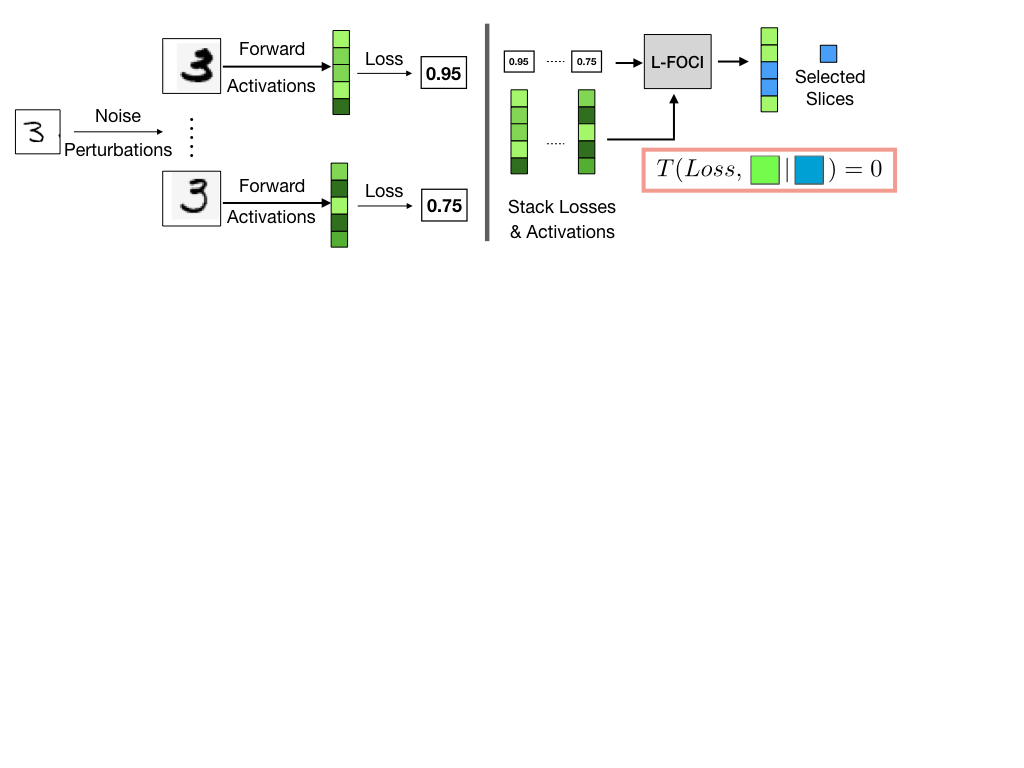
\includegraphics[width=\columnwidth,trim={0 18cm 4cm 0},clip]{5_unlearn/figs/foci_fig_new.png}
    % \vspace{-10pt}
    \caption[L-FOCI subset identification pipeline]{A sample is perturbed and passed through the network. Activations are aggregated alongside losses and fed to L-FOCI. Selected rows represent slices of the corresponding layer that are sufficient for unlearning.}
    \label{fig:lfoci}
\end{figure}

When using L-CODEC, we can use a more straightforward Markov Blanket identification procedure adapted from \cite{codec}. FOCI more directly selects which variables are valuable for explaining $z'$, and in fact, is proven to identify the sufficient set (Markov Blanket) with a reasonable number of samples. Briefly, in our L-FOCI, the sufficient set is built incrementally with successive calls to L-CODEC, moving the most ``dependent'' feature from the independent set to the sufficient set.
See Appendix~\ref{app:5:ci} for details.
% Additionally,they provide a simple procedure for sufficient subset selection, reproduced in Algorithm~\ref{alg:foci}.

\paragraph{Summary.} This procedure alleviates the first issue in terms of sufficient subset or Markov Blanket selection; compared to existing methods using information-theoretic measures that require permutation testing, L-FOCI directly estimates the change in variance when considering a proposal to add to the set.
Now, we discuss how this selection can help identify sets of parameters that can be updated.

\section{Deep Unlearning via L-FOCI Hessians}
%\section{Deep Unlearning via L-FOCI Hessians}
\label{sec:deepunlearn}

%As mentioned in Remark~\ref{rem:sens}, 
Our input samples to scrub $z^\prime$ are not random variables for which we have samples or distributional assumptions, nor are our parameters. In this case, 
% As mentioned in Remark~\ref{rem:sens},
a perturbation-based scheme may be useful when attempting to generate samples for unknown distributions.
% We take advantage of this directly to generate samples for any model context.

Considering Assump.~\ref{assum:sub}, when only some parameters are useful for the final outcome on an input sample $z^\prime \in S$, the effect of those parameters can be measured through activations due to the forward pass of a model. We estimate the conditional independence test in \eqref{eq:assum} through activations as
\begin{align}
    f(z^\prime) \bot a_{\Theta\setminus P}^* | a_P^*,
\end{align}
where $a_P$ for some parameter subset $P \subseteq \Theta$ is defined as the linear activations generated by the forward pass through the model.
This formulation relates to a generalized version of the solution in \S3 of \cite{bullseye}, where conditional mutual information is estimated via feature mappings.

As an example, if a network has linear layers $\cL$, a simple linear layer $l \in \cL$ with parameters $w_l \in \RR^{a \times b}$ would have activations $a_l \in \RR^b$, with $a_l = w_l a_{l-1}$. For each entry $a_{l,j}$ in the vector $a_l$, the associated parameters in the layer are $w_l[:,j]$. Thus, we break up the network into influential \textit{slices.} These slices can be seen as a finer view of the parameter space compared to typical layerwise selection, but coarser than a fully discrete one. Next, $\cL$ now refers to the collection of these slices, with a specific slice as $l$.

The tuple of variables we need samples from is now
\begin{align}
    \{a_1, \ldots a_{|\cL|}, \cL(z^\prime)\}
\end{align}
We can obtain samples from this set by perturbing the input and consecutively collecting activations along all weight slices during the computation of the loss. For a particular perturbation $\xi^j \sim N(0,\sigma^2)$,
\begin{align}
    x_i^j = x_i + \xi^j; \quad
    l^j, a_L^j = \{l(x_i^j), a_1^j, \ldots a_{|\cL|}^j\}
\end{align}
The tuples $(l^j, a_L^j)$ serve as samples for our conditional independence test, 
\begin{align}
    (P \subseteq \Theta) &= \mbox{L-FOCI}((l^j, a_\cL^j)_{j=1}^m)
\end{align}
for $J:=\{j \in 1,\ldots,m\}$ perturbations (see Figure~\ref{fig:lfoci}).

In Alg.~\ref{alg:blockunlearn}, the activations are collected using hooks within the forward pass. 
First, gradients at the last and penultimate epoch for full training are stored during the original training pass. Given a sample to unlearn, we compute L-FOCI over the perturbed activations and losses generated by the forward pass, and identify which parameter sets will be updated. We compute the approximate Hessian over these parameters via finite differences for both the full model and for the model only over the sample of interest. Finally, we apply the blockwise Newton update to the subset of parameters as in \eqref{eq:unlearn} with appropriate DP noise as in \cite{sekhari2021remember}.
\begin{algorithm}
\small
\SetAlgoLined
\KwData{A trained model $\hat{w}$, gradient vectors $\nabla_1 F(\hat{w}), \nabla_2 F(\hat{w})$, sample $z' \in \cS$ to unlearn.}
\KwResult{model $w'$ with $z'$ removed.}
1. \For{$j \in \{1,\ldots, m\}$ perturbations}{
    $\xi^j \sim N(0,\sigma^2)$ \\
    $z^{\prime,j} = z^\prime + \xi^j$ \\
    $l^j, a^j = f(z^{\prime,j})$ \\
    % \eIf{$T(z',w_{\setminus P}, w_{P \cup p}) < 0$}{break}{Append $P = P \cup p$}
}
2. Compute $P* = \mbox{L-FOCI}(l^J, a^J)$. \\
3. Compute $\nabla^2_{P} F(\hat{w}, z^\prime)$ via finite differences. \\
4. Update:
\begin{align}
    H_P' &= \frac{1}{n-1}\left(n \nabla^2_{P} F(\hat{w}) - \nabla^2_{P} f(\hat{w}, z')\right) \\
    w_{P}' &= \hat{w}_{P} + \frac{1}{n-1}H_{P}'^{-1} \nabla f(\hat{w}, z')_{P} \\
    w'_{\Theta\setminus P} &= \hat{w}_{\Theta\setminus P}
\end{align}
 \caption{\label{alg:blockunlearn} Unlearning via Conditional Dependence Block Selection}
\end{algorithm}

\paragraph{Computational Gains.}
A direct observation is that now we are doing sampling, which adds a linear computational load.
However, directly updating all parameters requires $O(d^3)$ computation due to matrix inversion, while this procedure requires $O(md + dm\log m + p^3)$, for the forward passes, FOCI algorithm, and subsequent subsetted matrix inversion. For any reasonable setting, we have $p \ll d$, and so this clearly offers significant practical advantages.








% Based on the above observations we make the following assumption for samples in the training set:
% \begin{assumption}\label{assum:sub}
% For all subsets of samples $S \subset D$, there exists a subset of the model parameters $P \subset \Theta$ such that 
% \begin{align}
%     L(S) \bot w_{\Theta\setminus P}^* | w_{P}^*
% \end{align}
% \end{assumption}

% \begin{assumption}
% \begin{align}
%     \forall S \sim \mathcal{P}(\mathcal{X}, \mathcal{Y}) \quad \exists T \subset L \\
%     s.t., \quad \mathcal{L}(S) \bot w^{*}_{L\setminus T} | w^{*}_T
% \end{align}
% \end{assumption}
% where, $S$ is the set of data points sampled from the joint training distribution of $\mathcal{P}(\mathcal{X}, \mathcal{Y})$, $w^*$ are the model parameters for a trained converged model, $L$ is the set of all layers (filters), $T$ is the subset of all layers which we will later tie to our selection algorithm. $\mathcal{L}$ is the loss function. 
% Note: $S$ can be a singleton containing only one data point to be removed. It is most beneficial to think of $S$ as a set of data points belonging to a particular class. 

% Input perturbation to get samples for FOCI computation: Given a data point $(x_k, y_k)$ from the training set $D$ we want to remove it. So, we perturb the input by adding small amount of Gaussian noise to generate samples for it. We have,

% \begin{align}
%     (x_k, y_k) \in D \xrightarrow[\text{perturbation}]{\text{input}} \{(x_k +g_k, y_k) | g_k \sim \mathcal{N}(0,1)\} = S_k
% \end{align}
% So, $S_k$ becomes our set S in \textbf{Assumption 1}. We generate sample for FOCI of the form $(\mathcal{L}(S_{k_i}), w^*(S_{k_i}))$; where $S_{k_i}$ is the $i$th perturbation of $x_k$ from set $S_k$ and $\mathcal{L}(S_{k_i})$ is the loss for the corresponding perturbation. 
% After this $FOCI({(\mathcal{L}(S_{k_i}), w^*(S_{k_i})) | S_{k_i} \in S_k})$ gives us the required $T \subset L$ selection; i.e. selects $T$ out of $L$ layers in the model following \textbf{Assumption 1}. 

% For the samples in the training set:
% \begin{assumption}
% For all subsets of samples $S \subset D$, there exists a subset of the model parameters $P \subset \Theta$ such that 
% \begin{align}
%     L(S) \bot w_{\Theta\setminus P}^* | w_{P}^*
% \end{align}
% \end{assumption}



% \begin{theorem}
% The change in the activation of a layer $l_{i+1}$ after an update to a previous one is bounded as:
% \begin{align}
%     |l_{i+1}(\tilde{a}_i) - l_{i+1}(a_i)| \leq \frac{2ML^2m^2}{\lambda^3 n^2}
% \end{align}
% \end{theorem}
% \begin{proof}
% Let the output of the previous layer be given as $w_l * a_{l-1}$, and the scrubbed output be $\tilde{w}_l * a_{l-1}$. Then we can Taylor expand around the output of the next layer for the previous  $l_{i+1}(\tilde{w}_l a_{l-1})$:
% \begin{align}
%     l_{i+1}(\tilde{w}_l a_{l-1}) &= l_{i+1}((w_l + \Delta) a_{l-1}) \\
%     &= l_{i+1}(w_l a_{l-1}) + \nabla l_{i+1}(w_l a_{l-1}) \Delta + O(\Delta^2)
% \end{align}
% where $\Delta = \tilde{w}_l - w^*_l$, or the Sekhari update:
% \begin{align}
%     \Delta = \frac{1}{n+1}H^{-1} \nabla f(x_r).
% \end{align}
% The first-order term vanishes, because the gradient at the original point $w_l$ is 0 given that we've trained

% %For a specific parameter layer, the linear assumption allows us to use a form of convexity (?). 
% From Lemma 6 in Appendix C.1 of  \cite{sekhari2021remember}, we have that 
% \begin{align}
%     |w^* - \tilde{w}| \leq \frac{2mL}{\lambda n},
% \end{align}
% so 
% \end{proof}

% \begin{theorem}
% Residual Gradient norm
% \end{theorem}
% \begin{proof}

% \end{proof}
\subsection{Theoretical Analysis}
By definition, any neural network as described above is actually a Markov Chain: we know that the output of a layer is conditionally independent of the penultimate one given the previous one, and clearly a change in one layer will propagate forward through the rest of the network.
However, when trained for a task with a large number of samples, the influence or ``memory" of the network with respect to a specific sample may not be clear.
%, and when unlearning we would prefer to be liberal in how layers are selected to be scrubbed.
While the output of the layers may follow a Markov Chain, the parameters in the layers themselves do not, and their influence on a sample through the forward pass may be highly dependent or correlated.
Practically, we would hope that unlearning samples at convergence does not cause too much damage to the model's performance on the rest of the input samples.
% through these knock-on effects. 
Following traditional unlearning analysis, we can bound the \textit{residual gradient norm} to relieve this tension.
\begin{lemma}
The gap between the gradient residual norm of the FOCI Unlearning update in Algorithm~\ref{alg:blockunlearn} and a full unlearning update via \eqref{eq:sekhariunlearn},
\begin{align}
||\nabla F(w^-_{Foci},D')||_2 - ||\nabla F(w^-_{Full},D')||_2
\end{align}
shrinks as $O(1/n^2)$.
\end{lemma}
\begin{proof}
The full proof is in the appendix. Main idea: Because we only update a subset of parameters, the gradients for the remainder should not change too much. Any change to a selected layer only propagates to other layers by $1/n$, and a Taylor expansion about the new activation for that layer gives the result.
\end{proof}


\paragraph{How L-CODEC achieves acceleration for Unlearning?}
Sampling with weights proportional to the Lipschitz constant of individual filters/layers is an established approach in optimization, see \cite{gorbunov2020unified}. We argue that L-CODEC computes an approximation to optimal sampling probabilities.
%for updating purposes. 
Under a mild assumption that the sampling probabilities have \emph{full} support, it turns out that correctness of our approximate (layer/filter selection) procedure can be guaranteed for unlearning purposes using recently developed optimization tools, see \cite{gower2019sgd}. By adapting results from \cite{gorbunov2020unified}, we can show the following, summarizing the main result of our slice-based unlearning procedure.
\begin{theorem}\label{thm:fociconv}
Assume that layer-wise sampling probabilities are nonzero. Given unlearning parameters $\epsilon,\delta$, the unlearning procedure in Alg~ \ref{alg:blockunlearn} is $(\epsilon',\delta')-$forgetting where $\epsilon'>\epsilon,\delta'>\delta$ represent an arbitrary  precision (hyperparameter) required for unlearning. Moreover, iteratively applying our algorithm converges exponentially fast (in expectation) w.r.t. the precision gap, that is, takes (at most) $O(\log\frac{1}{\mathbf{g_{\epsilon}}}\log\frac{1}{\mathbf{g_{\delta}}})$ iterations to output such a solution where  $\mathbf{g_{\epsilon}} = \epsilon'-\epsilon>0,\mathbf{g_{\delta}}=\delta'-\delta>0$ are gap parameters.
\end{theorem}
Our result differs from Nesterov's acceleration: we do not use previous iterates in a momentum or ODE-like fashion; rather, here we are closer to primal-dual algorithms where knowing nonzero coordinates at the dual optimal solution  
%(better duality gap) 
can be used to accelerate primal convergence, see \cite{diakonikolas2019approximate}. Moreover, since our approach is \textit{randomized}, the dynamics can be better modeled using the SDE framework for unlearning purposes, as in \cite{simsekli2020fractional}. 
% In our implementation,
Here, we do not  compute anything extra, although it is feasible for future extensions.
% And relate to additive error on $(\epsilon,\delta)$ forgetting in the beginning...
\begin{remark}
Our approach to estimate the Lipschitz constant is different from \cite{fazlyab2019efficient} where an SDP must be solved -- quite infeasible for unlearning applications. Our approach can be interpreted as solving a simplified form of the SDP proposed there, when appropriate regularity conditions on the feasible set of the SDP are satisfied. %constraint qualification assumptions.
\end{remark}

\paragraph{A note on convexity.}
Existing methods for guaranteeing removal and performance depend on models being convex. Practical deep learning applications however involve highly nonconvex functions.
The intuitions of unlearning for convex problems \textbf{directly apply to nonconvex unlearning} with one more technical assumption: minimizers of the learning problem satisfy Second Order Sufficiency (SOS) conditions. 
SOS guarantees that $ \nabla^2\hat{F}(\hat{w})$, $\hat{H}$ in eq (7) of [28] are PSD, and that the update (8) is an \textit{ascent} direction w.r.t. the loss function on $U$, making unlearning possible. Guarantees for nonconvex unlearning involve explicitly characterizing a subset of SOS points (so-called  ``basin of attraction" of population loss), i.e., which points gradient descent can converge to, see \S1.3 in \cite{Traonmilin_2020}. 
%
%In fact, in some nonconvex signal  processing applications, it is possible to explicitly specify global minima (satisfies SOS) of the population loss by characterizing  ``basin-of-attraction" of the empirical minimizer, see Section 1.3 in \cite{traonmilin2020basins}  i.e., points that gradient descent can converge to. 
So, will minimizers from first order methods satisfy SOS conditions? Generally, this is not true, e.g., when the Hessian is indefinite, $\hat{H}\not\succeq 0$, the update itself may not be an ascent direction w.r.t. negative of the loss. Here, standard Hessian modification schemes are applicable \cite{wright1999numerical}, subsequently using the Newton's step in \cite{sekhari2021remember} with a diagonally modified Hessian.


% While better nonconvex guarantees and algorithms are still open problems for general unlearning, here, 
We fix weight decay during training, acting as $\ell_2$ regularization and giving us an approximate $\lambda$-strong convexity. We also take advantage of this property to smooth our Hessian prior to inversion, intuitively extending the natural linearization about a strongly-convex function. Interestingly, this exactly matches a key conclusion from \cite{basu2021influence}: weight-decay heavily affects the quality of 
the measured influence,  
consistent with our nonconvexity discussion.
% Also, it {\bf exactly matches} our practical adjustments via adding $\ell_2$ regularization (L563, page 6)!
% We enables analysis like in Basu et al. for large scale problems. There,
% using tools from Hessian inverse estimation only allows evaluating metrics on few potentially ``influential" samples. Our scheme within Basu et. al. can enable influence estimation for all samples. 

% All models are trained using a weight decay of $0.01$, corresponding to $l_2$-regularization and $\lambda$-strong convexity as needed by the traditional update in \cite{sekhari2021remember}. 
% breaking ties randomly, leads to constants,
% add small noise to break ties, constants go away
% tie breaking is hard? faster when added noise










%%%%%%%% old



%\subsection{Efficient Computation via Blockwise Hessian Selection}

% Let the set of layers be $\cL$, whose size is the number of layers in the network of interest, and let a subset of the weights for a set $L \subseteq \cL$ be $w_L$. In this case we use the term layers loosely; a convolutional block may have a number of filters that can be considered separately.



%These matrices can be quite large, and additionally require updating all weight parameters.

%However, if we can effectively determine the Markov Blanket of the parameters that, when conditioned upon, make the rest irrelevant, we could reduce the number of parameters that need to be updated, and additionally reduce the computation needed for those updates. We can consider the parameters in groups by layers, and potentially attack from a blockwise perspective.

%Let the set of layers be $\cL$, whose size is the number of layers in the network of interest, and let a subset of the weights for a set $L \subseteq \cL$ be $w_L$. 

% Denote the layers of the network that define the conditionally sufficient set as $w_{L^*}$ for a sample $z_i$ where $L^* \subseteq \cL$. Analogous to Eq.~\eqref{eq:paramCI}, we can write
% \begin{align}\label{eq:layerCI}
    % z \bot w_l | w_{L^*}, \ \forall l \in \cL\setminus L^*.
% \end{align}



% \begin{remark}
% Directly applying FOCI as above still leads to large computation costs when millions of parameters make up the potential sufficient set. However, we can take advantage of structured observations made by others, analogous to group lasso schemes in linear models. Particularly, recent work has observed networks behave similarly within {\em blocks} \cite{bau2017network,fong2018net2vec}.
% % Intuitively, we may expect that \textit{blocks} of parameters may demonstrate independence to specific samples together \cite{???}.
% In a large convolutional neural network, specific filters learned for separating the input space may only be active for specific types of inputs; on others they may be completely ``off". We take advantage of this in the next section.
% \end{remark}
% This angle also provides a nice perspective on explainability through independence, which we examine in the experiments.

% \subsection{Identifying CI Layers via Hypercolumn Representations}\label{sec:hyper}
% Computing the test in \ref{eq:layerCI} is not so straightforward. The parameters themselves are not random variables, and while ``samples" 
% How can we compute the independence above?
% We can approximate the independence of the parameters by the independence of the feature activations at that layer.

% Define the activations of a sample $x$ as $H(x)$, defined as the set of activations after each linear parameter layer in the model.

% We estimate the above CI test through the activations:
% \begin{align}
%     z \bot h(z)_l | h(z)_{L^*}, \ \forall l \in \cL\setminus L^*
% \end{align}
% This formulation is related to a generalized version of the solution presented in Section 3 of \cite{bullseye}, where conditional mutual information is estimated via feature mappings.

% \paragraph{Random variable instances.} Using hypercolumn representations, we can directly instantiate each pixel (or feature) of the layers as an instantiation of that layer. Specifically, the tuples $(z_{ij}, h(z)_{l,ij})$ become our samples for estimating L-CODEC among the random variables $(z,h(z))$. 

% Now have a drastically reduced computation scheme. First, we run FOCI on hypercolumn feature maps to select CI layers (or filters). Next, we Update weights with the traditional Hessian update (now feasible) on only those layers.

% With Hypercolumn interpolation, for deep convolutional layers size expansion may lead to large constant regions in exploded image. Traditional CODEC calls would randomly tie break, causing variance in the measure to be very high, even though we know that taking expectation of this randomness would lead to low/zero CODEC values. This may also be the case when testing data that lies in a set $S \subseteq \RR$, such as binary attributes or other data with some discrete but ordinal structure. For this reason a direct application of the statistic in \cite{codec} is not feasible, and it is necessary to apply our randomized version in Eq.~\eqref{eq:lcodec}.

% This setup also provides some form of model explainability. Identifying the layers (or filters) of the that are conditionally independent also rep


%Ablations below show this does not significantly effect identifying dependence via CODEC directly, nor downstream use.

%\subsection{Hessian Estimation}
%The vanilla unlearning algorithm in \cite{} proceeds as follows. First, the ERM estimate of the parameters are computed in typical fashion over the entire dataset $S := \{z_i\}_{i=1}^n \sim \cD^n$
%\begin{align}
%    \hat{w} = \arg\min_w \hat{F}(w) := \frac{1}{n}\sum_{i=1}^n f(w,z_i),
%\end{align}
%and the weights $\hat{w}$ and the Hessian at the minimizer $\nabla^2\hat{F}(\hat{w})$ are returned.

%Next, for a set of ``delete requests" $U := \{z_i\}_{i=1}^m \subseteq S$, the unlearning step makes use of an intermediate Hessian in the form of:
%\begin{align}
%    \hat{H} = \frac{1}{n-m}\left(n\nabla^2\hat{F}(\hat{w}) - \sum_{z\in U} \nabla^2 f(\hat{w}, z)\right),
%\end{align}
%and an update step of 
%\begin{align}
    %\bar{w} = \hat{w} + %\frac{1}{n+m}(\hat{H})^{-1} \sum_{z\in U} \nabla f(\hat{w},z)
%\end{align}
%With noise sampled from a Normal with variance as a function of the smoothness of the loss $f$ and the number of samples.

% Our final procedure for efficient unlearning works as follows, summarized in Algorithm~\ref{alg:blockunlearn}. First, gradients at the last and penultimate epoch for full training are stored. Given a sample to unlearn, we compute L-FOCI over the hypercolumn generated by the forward pass, and identify which parameter sets will be updated. We compute the approximate Hessian over these parameters via finite differences for both the full model and for the model only over the sample of interest. Finally, we apply the blockwise Newton update to the subsetted parameters as in Eq.~\eqref{eq:unlearn}.
% \begin{algorithm}
% \SetAlgoLined
% \KwData{A trained model $\hat{w}$, gradient vectors $\nabla_1 F(\hat{w}, \nabla_2 F(\hat{w})$, sample $z' \in \cS$ to unlearn.}
% \KwResult{model $w'$ with $z'$ removed.}
% 1. Perform a forward pass of the model with $z'$. \\
% 2. Construct the hypercolumn $h(z')$ of $z'$. \\
% 3. Compute L-FOCI($z', h(z')$) to identify the filters $L^*$ to update. \\
% 4. Compute $\nabla^2 F(\hat{w})$ as the finite difference of $\nabla_1 F(\hat{w}), \nabla_2 F(\hat{w})$.\\
% 5. Update:
% \begin{align}
%     H_L' &= \frac{1}{n-1}\left(n \nabla^2_L F(\hat{w}) - \nabla^2_L f(\hat{w}, z')\right) \\
%     w_L' &= \hat{w}_L + \frac{1}{n-1}H_L'^{-1} \nabla f(\hat{w}, z')_L \\
%     w'_{\setminus L} &= \hat{w}_{\setminus L}
% \end{align}
%  \caption{\label{alg:blockunlearn} Unlearning via Conditional Dependence Block Selection \ronak{switch from hypercol to activation maps}}
% \end{algorithm}
\paragraph{Implementation Details.}
As we only need a subset of the Hessian, we compute the finite difference among the parameters within the blocks selected.
For large models, even subsets of model parameters may lead to large Hessian computations, so we move parameters as needed to the CPU for parameter updates. Pairwise distance computations for CI testing via nearest neighbor are carried out on the GPU \citep{yoso-zhanpeng}.
Our code, achieves reasonable run-time for unlearning for deep models, e.g., one unlearning step for a person re-identification task on a ResNet50 model with roughly 24M parameters takes about 3 minutes.  

% compute hessians/gradients as concatenated vectorized versions of gradient lists stored as above.

% gamma-learnability important; if the model is not trained fully (close to optimal) then it doesn't work.

% model size is an important piece

\begin{figure}[t]
\vspace{-0.1in}
    \centering
    \raisebox{\baselineskip}%
    {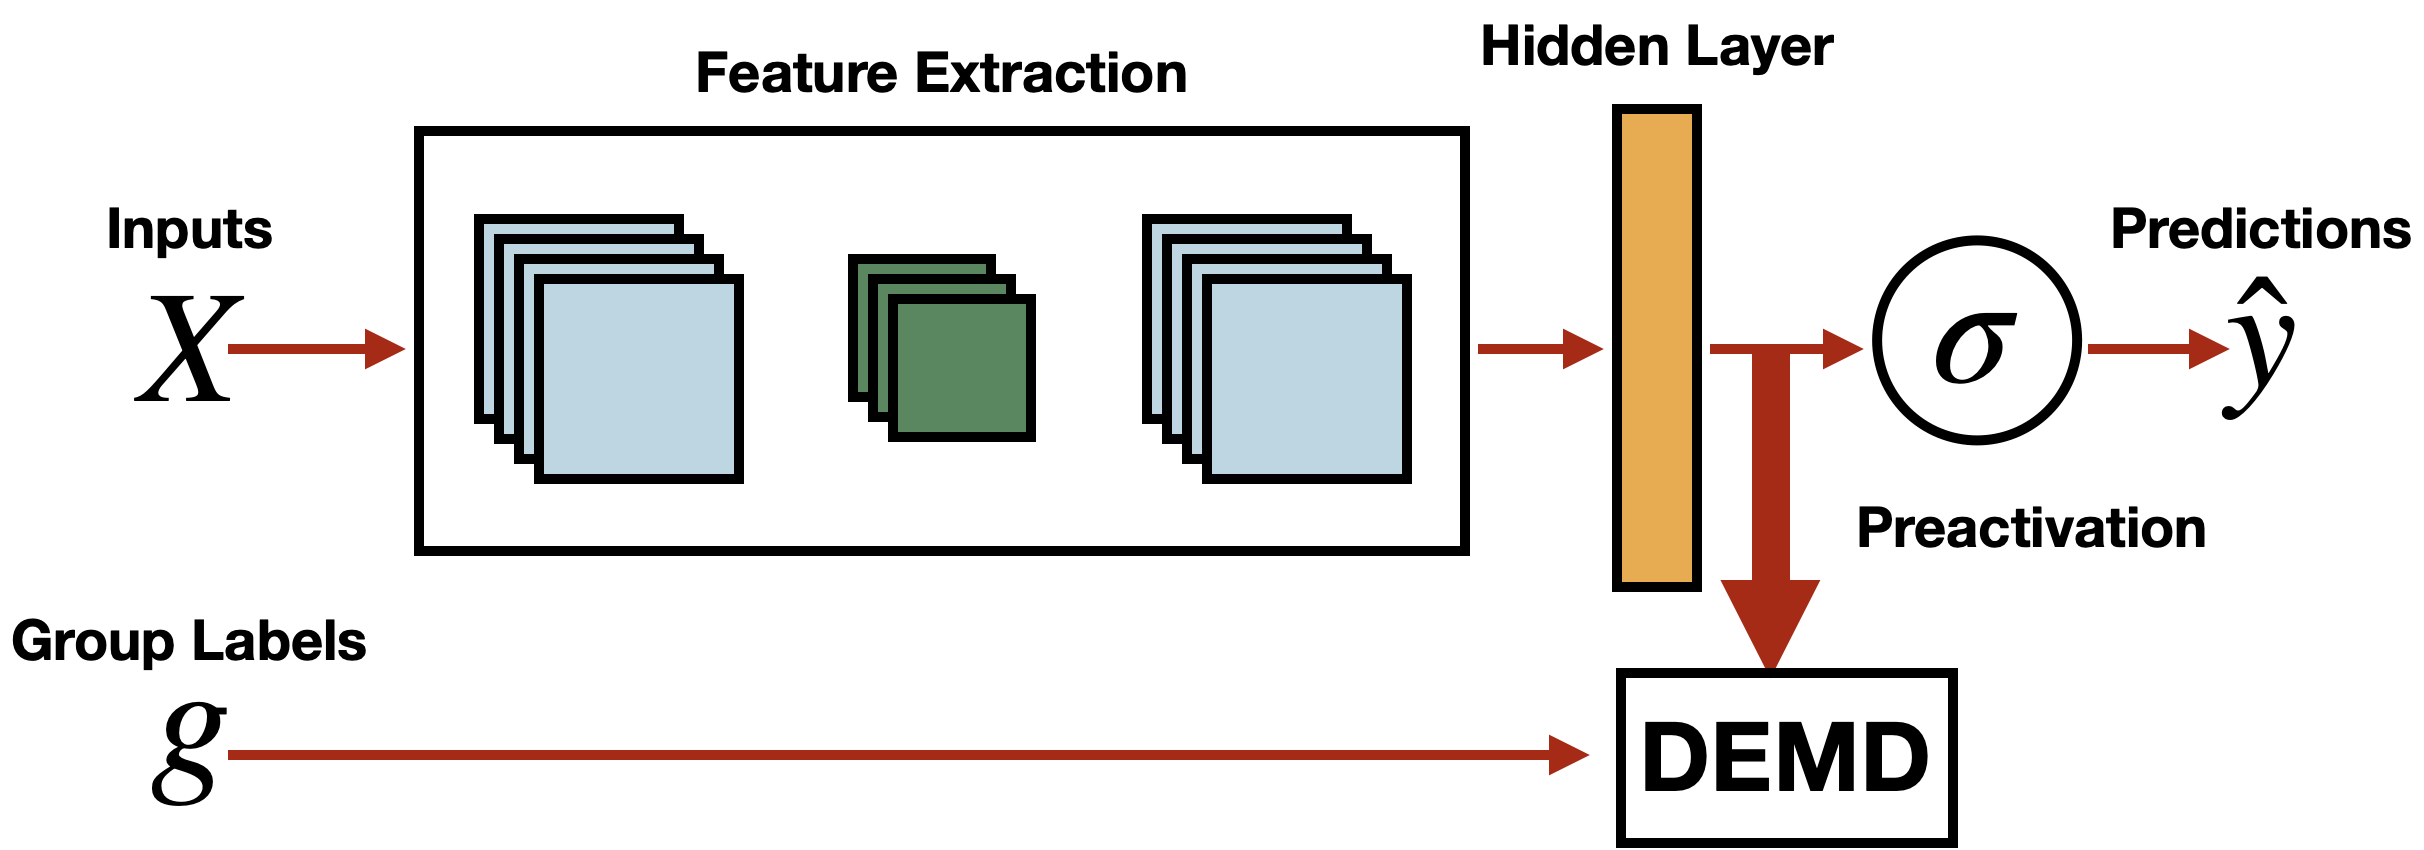
\includegraphics[width=0.55\columnwidth]{6_demd/figs/net_diff_new.png}%
    }% 
    \;
    \includegraphics[width=0.35\columnwidth]{6_demd/figs/Distance_Comparisons.pdf}
    \vspace{-10pt}
    \caption{\footnotesize \label{fig:dists} (Left) DEMD is positioned after the final layer, prior to the activation. Activations are sorted into distributions utilizing group labels provided alongside the input data. Computed distributions are then brought together using our algorithm. (Right) Computation times for direct distance evaluation of EMD-like distances. Existing methods take much more time {\color{blue}(check $y$-axis)} as the number of distributions grow.}
    \vspace{-5pt}
\end{figure}

\section{Experiments}
\label{sec:results}
\vspace{-5pt}
% \subsection{Implementation Details}
% While accounting for dual variables in practice is relatively easy, we may directly take advantage of existing automatically computed gradients from existing software to avoid the bookkeeping and tracking of dual variables entirely. While these gradients may not exactly equal the dual variables, they are directions of descent with respect to our distributions of interest, and are equally sufficient for our purposes.

% Traditional analysis and learning pipelines do not consist of binned distributions, but rather empirical distributions over real-numbered outputs. For this reason it is necessary that we construct a differentiable histogramming operation, that will allow gradients computed with respect to the dEMD measure to flow backwards on a per-sample or per-batch basis. 

% \vishnu{I feel these details are not necessary in the main paper. } Experiments were conducted using NumPy and PyTorch on a Intel(R) Xeon(R) CPU E5-2620 v3 @ 2.40GHz with an Nvidia Titan Xp GPU. 
We evaluate our construction in a number of settings. 
First, we demonstrate the computational speedup associated with evaluating d-MMOT using our algorithm, along with speedups associated with directly computing the gradient.
Next, we compute the construction in a series of neural network tasks associated with ensuring distributional similarity: fairness, invariant representations, and multi-domain matching.
We provide a complete PyTorch Network Module that packages the above differentiable DEMD objective and histogram functions,
and serves as a plug-and-play regularization module. Code is available in the supplement. %\vishnu{One major criticism in the experiments is we don't evaluate in a setting where there are too many distributions to match. }


\subsection{Performance Benchmarks}

Figure \ref{fig:speeds} presents NumPy and Torch instantiations of both forward and backward passes using automatic differentiation and the gradients computed using the dual as in \S\ref{sec:dual}. As expected, the forward (distance computation) times are comparable, but the backwards computation scales poorly with the number of distributions to be updated using automatic differentiation. Our dual setting allows the gradients to simply be read off (based on the forward pass), leading to \textbf{no} additional computation overhead during backpropagation.
\begin{figure}[ht]
    \centering
    \fbox{
    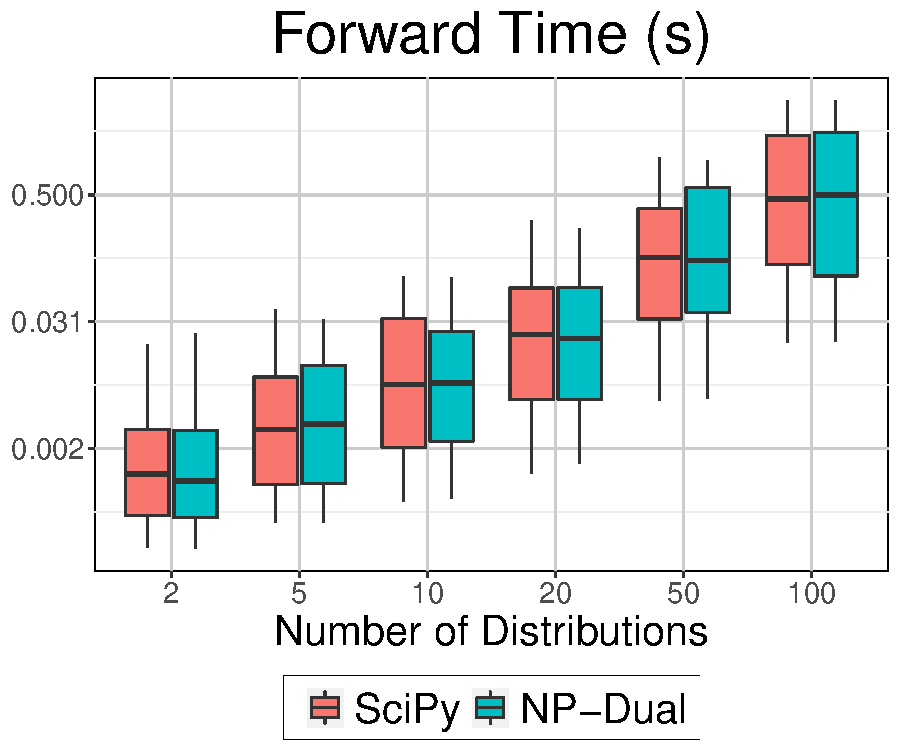
\includegraphics[width=0.22\textwidth]{6_demd/figs/fwbk_new/Numpy_Forwards_10Bins.pdf}
    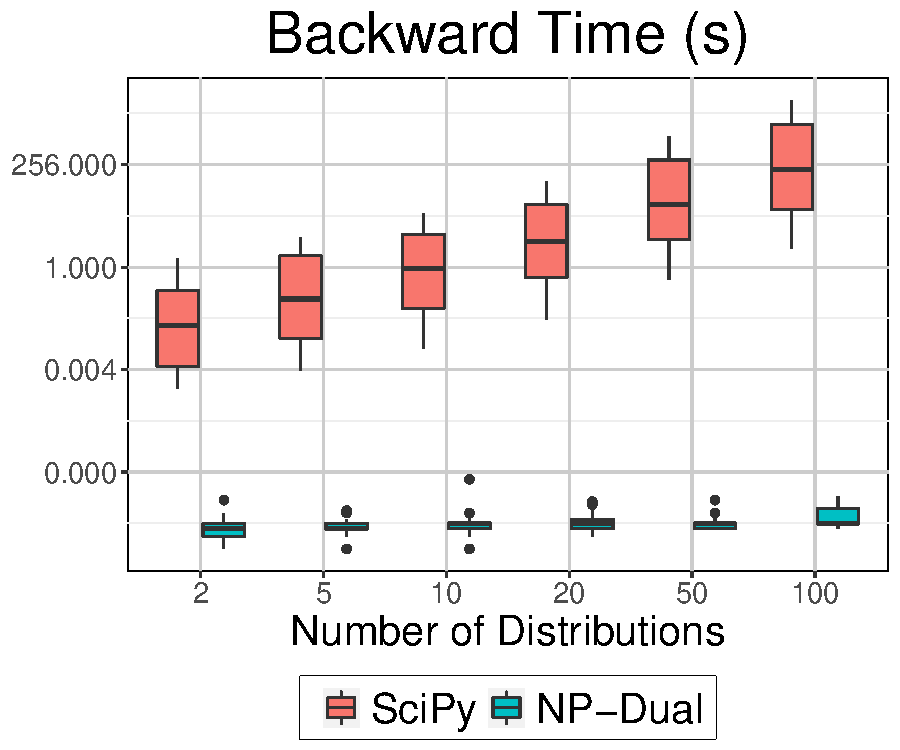
\includegraphics[width=0.22\textwidth]{6_demd/figs/fwbk_new/Numpy_Backward_10Bins.pdf}
    }%
    \;
    \fbox{
    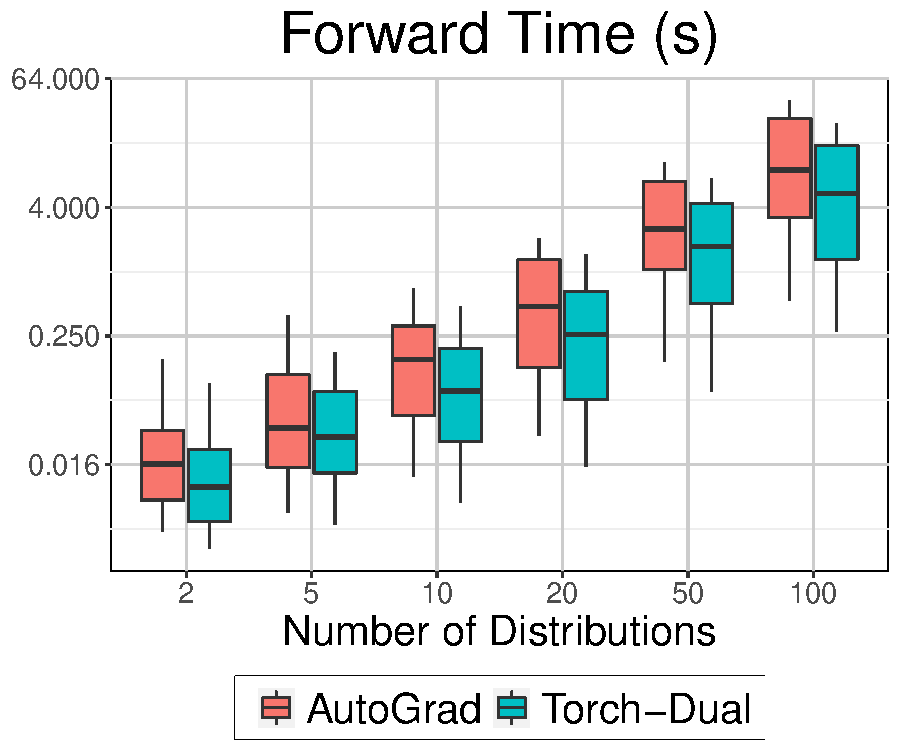
\includegraphics[width=0.22\textwidth]{6_demd/figs/fwbk_new/Torch_Forwards_10Bins.pdf}
    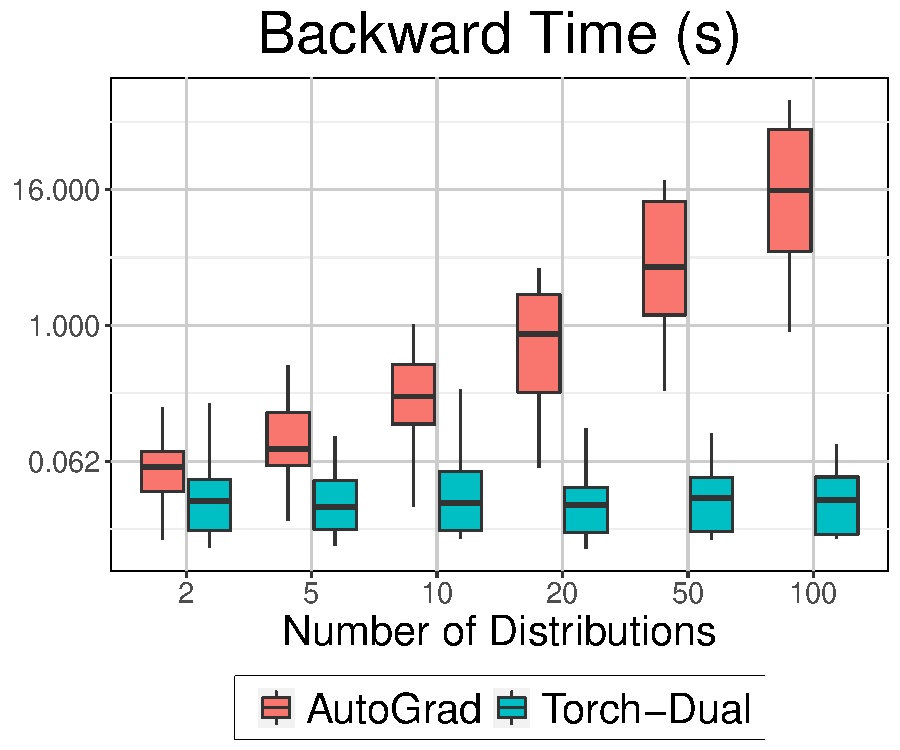
\includegraphics[width=0.22\textwidth]{6_demd/figs/fwbk_new/Torch_Backward_10Bins.pdf}
    }%
    \caption{\footnotesize Forward/Backward Pass Times for 10 Bins with varying number of distributions, averaged over 10 runs. Forward wall-clock times are comparable, regardless of backend ({\em left pair}: NumPy+SciPy; {\em right pair}: PyTorch+AutoGrad). Direct reading of the gradient via the dual leads to significant gains in backward pass times, where automatic differentiation scales poorly with the number of distributions.}
    \label{fig:speeds}
    \vspace{-5pt}
\end{figure}


% \subsection{Comparing Methods for Optimal Transport with Monge Metrics}
We compare our DEMD computation 
%of the Earth Mover's Distance 
to what one may use given existing Optimal Transport methods in Figure \ref{fig:dists} (right). Using standard off-the-shelf methods as a baseline, when the cost is Monge our algorithm provides \textit{significant} speedups in computation time, on the scale of orders of magnitude! Further, if the number of distributions and bins increases, the time-cost for existing methods using more generic LP solvers can become significant, and may become infeasible with generic solutions via CVXPY \citep{diamond2016cvxpy}. 
% Figure \ref{fig:dists} shows the time dependence as the number of distributions grows, with 10 bins. 
We compare our approach to two off-the-shelf implementations of barycenters via the Python Optimal Transport (POT) Library \citep{flamary2021pot}, along with 
directly solving the Earth Mover's problem via CVXPY. 
Even for 10 distributions over 10 bins, CVXPY is unable to allocate the necessary memory using a direct instantiation.

% \begin{figure}
%     \centering
%     \includegraphics[width=0.45\columnwidth]{figs/Distance_Comparisons.pdf}
%     \caption{Times for direct distance computation of EMD-like distances. See text for details.}
%     \label{fig:dists}
% \end{figure}

%% Barycenters doesnt work right now
% \subsection{Common Barycenter Computations and Comparisons}
% -comparing with Cuturi and janati here, working on setup with janati code

% \begin{figure}
%     \centering
%     \includegraphics[width=0.8\columnwidth]{example-image-a}
%     \caption{Comparison of approaches against DEMD over ellipse barycenters.}
%     \label{fig:}
% \end{figure}


%\section{Traditional methods for optimizing fairness: How do we compare?}
% \subsection{Example Applications}
% Here we instantiate the full setting as described in Section \ref{sec:fair}, and compare to existing drop-in regularizers meant to account for fairness. Because our approach operates on the activations prior to classification, we first compare our method using only two bins defined as above or below 0.5, so as to directly mimic the classification metric used in existing setups.

% \subsection{MNIST}
% Using the MNIST handwritten digit dataset, we construct a new classification problem. The distribution of digit size within the frame is typically the same; we augment the dataset with ``small" and ``large" versions of the digits within a single frame, and define a classification problem over determining the size of the digit within the frame. An ideal size classifier in this case should be agnostic to the digit being classified as large or small.

% \begin{figure}
%     \centering
%     \includegraphics[width=0.8\columnwidth]{example-image-b}
%     \caption{Effect of varying DEMD regularization weight, accuracy across groups.}
%     \label{fig:mnist}
% \end{figure}

\subsection{Generalized EM Fairness on Fairness Datasets}
With a viable tool in hand, we move to practical applications in machine learning fairness,
which naturally requires
enforcing closeness in model outputs.
Here, we construct networks with our DEMD regularizer,
where we discretize the final activation output
prior to classification,
and push the distributions of this activation to be similar
among sensitive attributes.

{\bf Data.}
We identify 4 common fairness datasets often used to benchmark
fair machine learning algorithms: (1) the German Credit Dataset \citep{german}, (2) the Adult Income Dataset \citep{uci}, (3) the Communities and Crime Dataset \citep{crime}, and (4) The ACS Income dataset, recently made available as a large, population-level demographic dataset \citep{ding2021retiring} containing as many as nine sensitive attributes. We set up a simple three-layer neural network for classification tasks with the addition of a fairness-type regularizer. We compare our construction with 4 off-the-shelf plug-in regularizers: (1) No regularization, (2) Demographic Parity (DP), (3) Equalized Odds (EO), and (4) a histogrammed barycenter construction. DP and EO regularizers were computed using a PyTorch version of FairLearn \citep{bird2020fairlearn}, and the barycenter version was implemented using POT library (with GPU backend). Because the scale of the regularization term is not directly comparable, we sweep regularization weights and select the best over all measures for a each dataset/regularizer pair. 
We use 10 bins and replicate all experiments over three random seeds.

% The American Census Survey (ACS) has recently made available a large set of demographic data. The original UCI Adult dataset \cite{uci} was curated from this data, however recent work by \cite{ding2021retiring} has identified temporal shifts in demographic data, and recommends using a more recent collection as a baseline when evaluating biases and adjusting for fairness. Part of their contribution includes APIs to directly interface with the data provided by the ACS, and the ability to identify and construct similar problems associated with the original UCI-provided dataset, albeit with updated data. Data for the income prediction task was downloaded from 2018, localized to California. After preprocessing, 195665 samples were split: 75\% training and 25\% validation. Race is the provided group label, which we wish to be agnostic toward over some measure of our output.
{\bf Models.} We set up two model settings with a standard logistic regressor and a 2-layer neural network. We compare three types of plug-in regularizers: (1) Demographic Parity (DP), (2) Equalized Odds (EO), and (3) the Generalized EMD. DP and EO regularizers were computed using a PyTorch implementation of FairLearn \citep{bird2020fairlearn}. 
%Since the scale of the regularization term in our measure is not directly comparable, we sweep over the regularization weights. 

{\bf Results.} In the summary in Table~\ref{tab:fair_results}, models were selected with the largest regularization weight before accuracy dropped significantly. When accuracies are comparable, we see good performance (when minimizing DEMD regularizer) against baseline methods. Notably, when accuracies are similar across methods, minimizing DEMD tends to give better (lower) fairness measures across all datasets.
{\bf Summary:} DEMD on the final network layer helps control multiple fairness measures.


% First we see that sweeps over regularization weights act as expected for our metric, as well as for existing fairness measures. 
% Table~\ref{tab:acsinc2} show results after training with a large range of regularization weights.
% Training models with no regularization leads to significantly different accuracies over race groups within the data, and strong regularization reduces both the EMD distance and traditional fairness measures over the output via demographic parity (DP) and equality of opportunity (EO). Table~\ref{fig:reg_sweep} shows a particular tighter sweep for EMD regularizer with 10 bins used as the discretization level, closer to the region with large swings in the trade-off. Close correspondence with DP and EO measured after thresholding suggests the model may be robust to choices in the selection threshold.
% Validation results for various models and regularization weights on the ACS Income prediction task including demographic parity
% (DP) and equality of opportunity (EO) spreads. In this setting only two bins are used for direct comparison to output-style regularizers.


\begin{table*}[!t] 
	\scriptsize
	\setlength\tabcolsep{3.5pt} % make LaTeX figure out width of inter-column spaces
	\caption{\footnotesize \textbf{Fairness Experiments.} Measures evaluated using standard metrics: maximum Demographic Parity Gap \textbf{(DP)},  maximum Equalized Odds Gap \textbf{(EO)}, and \textbf{(DEMD)}. For all measures, lower values are preferred.  With comparable accuracy, DEMD regularization leads to fairer representations as measured by common metrics. DP and EO measures are scaled by 100 for ease of presentation. Best results shown in bold.}
	\vspace{-10pt}
	\begin{tabular*}{\linewidth}{l *{3}{c}|*{3}{c}|*{3}{c}|*{3}{c}}
		\midrule%\midrule
		& \multicolumn{3}{c}{German} & \multicolumn{3}{c}{Adult} & \multicolumn{3}{c}{Crime}& \multicolumn{3}{c}{ACS-Income} \\
		\cmidrule{2-4} \cmidrule{5-7} \cmidrule{8-10} \cmidrule{11-13}
		& DP & EO & DEMD & DP & EO & DEMD & DP & EO & DEMD & DP & EO & DEMD \\ 
		\midrule
% 		None & 0.180 & 0.134 & 1.694 & 0.382 & 0.446 & 2.858 & 0.351 & 0.306 & 3.556 & 0.365 & 0.251 & 4.778 \\
% DP-Reg. & 0.169 & 0.128 & 1.600 & 0.383 & 0.446 & 2.832 & 0.362 & 0.250 & 3.705 & 0.477 & 0.276 & 5.024 \\
% EO-Reg. & 0.143 & 0.116 & 1.425 & 0.377 & 0.442 & 2.830 & 0.363 & 0.311 & 3.055 & 0.377 & 0.256 & 4.818 \\
% Bary & 0.177 & 0.134 & 1.645 & 0.362 & 0.442 & 2.811 & 0.377 & 0.256 & 2.726 & 0.571 & 0.497 & 4.376 \\
% DEMD & 0.145 & 0.117 & 1.443 & 0.364 & 0.438 & 2.688 & 0.288 & 0.361 & 3.101 & 0.334 & 0.236 & 3.598 \\
None & $17\scriptscriptstyle(5)$ & $11\scriptscriptstyle(2)$ & $1.69\scriptscriptstyle(0.32)$ & $18\scriptscriptstyle(1)$ & $13\scriptscriptstyle(0)$ & $1.69\scriptscriptstyle(0.07)$ & $38\scriptscriptstyle(6)$ & $45\scriptscriptstyle(3)$ & $2.86\scriptscriptstyle(0.38)$ & $37\scriptscriptstyle(1)$ & $25\scriptscriptstyle(0)$ & $4.78\scriptscriptstyle(0.32)$ \\
DP-Reg. & $16\scriptscriptstyle(6)$ & $10\scriptscriptstyle(3)$ & $1.5\scriptscriptstyle(0.26)$ & $17\scriptscriptstyle(1)$ & $13\scriptscriptstyle(1)$ & $1.6\scriptscriptstyle(0.07)$ & $38\scriptscriptstyle(6)$ & $45\scriptscriptstyle(3)$ & $2.83\scriptscriptstyle(0.39)$ & $48\scriptscriptstyle(4)$ & $28\scriptscriptstyle(0)$ & $5.02\scriptscriptstyle(0.31)$ \\
EO-Reg. & $17\scriptscriptstyle(5)$ & $11\scriptscriptstyle(2)$ & $1.69\scriptscriptstyle(0.32)$ & $\textbf{14}\scriptscriptstyle(1)$ & $\textbf{12}\scriptscriptstyle(1)$ & $\textbf{1.43}\scriptscriptstyle(0.07)$ & $38\scriptscriptstyle(5)$ & $\textbf{44}\scriptscriptstyle(3)$ & $2.83\scriptscriptstyle(0.39)$ & $38\scriptscriptstyle(1)$ & $26\scriptscriptstyle(0)$ & $4.82\scriptscriptstyle(0.32)$ \\
Bary-POT & $27\scriptscriptstyle(5)$ & $17\scriptscriptstyle(1)$ & $1.5\scriptscriptstyle(0.21)$ & $18\scriptscriptstyle(1)$ & $13\scriptscriptstyle(0)$ & $1.64\scriptscriptstyle(0.07)$ & $\textbf{36}\scriptscriptstyle(5)$ & $\textbf{44}\scriptscriptstyle(4)$ & $2.81\scriptscriptstyle(0.3)$ & $57\scriptscriptstyle(37)$ & $50\scriptscriptstyle(44)$ & $4.38\scriptscriptstyle(0.16)$ \\
DEMD (ours) & $\textbf{14}\scriptscriptstyle(7)$ & $\textbf{9}\scriptscriptstyle(4)$ & $\textbf{1.41}\scriptscriptstyle(0.35)$ & $15\scriptscriptstyle(1)$ & $\textbf{12}\scriptscriptstyle(1)$ & $1.44\scriptscriptstyle(0.08)$ & $\textbf{36}\scriptscriptstyle(6)$ & $\textbf{44}\scriptscriptstyle(3)$ & $\textbf{2.69}\scriptscriptstyle(0.44)$ & $\textbf{33}\scriptscriptstyle(0)$ & $\textbf{24}\scriptscriptstyle(0)$ & $\textbf{3.6}\scriptscriptstyle(0.29)$ \\
		\midrule%\midrule
	\end{tabular*}
	\label{tab:fair_results}
	%\vspace{-20pt}
\end{table*} 

\subsection{Harmonization for Invariant Representations}
Having evaluated the use of the DEMD layer to constrain the neural network for  fairness measures, we will now move to a more general problem of deriving invariant representations from the datasets. Here, invariance is sought in regard to the sensitive attributes. Recent works \citep{equivar} on invariant representation learning propose leveraging an encoder-decoder architectures to map the dataset features to latent space representations. The latent space representations are penalized to match or harmonize the distributions across several groups in the dataset. In contrast to the previous section, the goal here is to identify a good mapping in the latent space that is devoid of any group-related information in the dataset.  Consequently, our evaluation metrics test if the latent representations have a lower value of (i) ADV, adversarial measure and (ii) MMD, maximum mean discrepancy measure. The measure ADV tests to what extent can a separate neural network predict the group information from the latent features. Alternatively, the MMD scores measure the distance between the probability distributions across groups. Prior works such as \cite{zemel} and \cite{cai} optimize each of these measures separately. Our experiments (Table~\ref{tab:harm_results}) show the DEMD layer performs competitively with the baselines when applied on the latent space. Interestingly, these performance gains come despite not directly optimizing the harmonization measures, in contrast to baselines, which require several practical adjustments (batch variants and secondary neural networks).
\textbf{Summary}: DEMD as an intermediate layer can be used to derive invariant representations efficiently.
% \vishnu{Need to convey a message that the baseline directly optimizes for the ADV and MMD measures. Our although doesn't directly optimizes these measures, still achieves competitive values on them. }
%Due to skewness amongst the groups, ROC-AUC is used to report the ADV measure on German dataset.
\begin{table*}[!t] 
	\scriptsize
	\setlength\tabcolsep{2.25pt} % make LaTeX figure out width of inter-column spaces
	\caption{\footnotesize \textbf{Harmonization Experiments.} Evaluations conducted along three metrics, Accuracy \textbf{(ACC)}, Adversarial measure \textbf{(ADV)} and Maximum Mean Discrepancy \textbf{(MMD)}. A lower value $\downarrow$ of ADV and MMD indicate successful harmonization across the different groups. A higher ACC with a small drop from baseline is preferred. }
	\vspace{-10pt}
	\begin{tabular*}{\linewidth}{l *{3}{c}|*{3}{c}|*{3}{c}|*{3}{c}}
		\midrule%\midrule
		& \multicolumn{3}{c}{German} & \multicolumn{3}{c}{Adult} & \multicolumn{3}{c}{Crime}& \multicolumn{3}{c}{ACS-Income} \\
		\cmidrule{2-4} \cmidrule{5-7} \cmidrule{8-10} \cmidrule{11-13}
		& ACC $\uparrow$ & ADV $\downarrow$ & MMD $\downarrow$ & ACC $\uparrow$ & ADV $\downarrow$ & MMD $\downarrow$ & ACC $\uparrow$ & ADV $\downarrow$ & MMD $\downarrow$ & ACC $\uparrow$ & ADV $\downarrow$  & MMD $\downarrow$ \\ 
		\midrule
		None & $74\scriptscriptstyle(0.9)$ & $93\scriptscriptstyle(1.3)$ & $7.7\scriptscriptstyle(0.8)$ & $84\scriptscriptstyle(0.1)$ & $83\scriptscriptstyle(0.1)$ & $9.8\scriptscriptstyle(0.3)$ & $85\scriptscriptstyle(0.2)$ & $77\scriptscriptstyle(0.5)$ & $14\scriptscriptstyle(0.1)$ & $78\scriptscriptstyle(0.1)$ & $98\scriptscriptstyle(0.7)$ & $160\scriptscriptstyle(2)$ \\
		\cite{zemel} & $73\scriptscriptstyle(1.5)$ & $92\scriptscriptstyle(1.3)$ & $1.5\scriptscriptstyle(0.3)$ & $84\scriptscriptstyle(0.1)$ & $83\scriptscriptstyle(0.1)$ & $3.1\scriptscriptstyle(0.3)$ & $85\scriptscriptstyle(0.5)$ & $76\scriptscriptstyle(1.6)$ & $12\scriptscriptstyle(1.0)$ & $78\scriptscriptstyle(0.1)$ & $97\scriptscriptstyle(0.5)$ & $17\scriptscriptstyle(1.2)$ \\
		\cite{cai} & $76\scriptscriptstyle(1.3)$ & $93\scriptscriptstyle(0.6)$ & $1.2\scriptscriptstyle(0.2)$ & $84\scriptscriptstyle(0.04)$ & $81\scriptscriptstyle(0.7)$ & $4.2\scriptscriptstyle(2.4)$ & $85\scriptscriptstyle(0.2)$ & $76\scriptscriptstyle(0.7)$ & $15\scriptscriptstyle(0.6)$ & $78\scriptscriptstyle(0.1)$ & $94\scriptscriptstyle(5.6)$ & $99\scriptscriptstyle(2.9)$ \\
		DEMD (ours) & $74\scriptscriptstyle(1.1)$ & $93\scriptscriptstyle(0.4)$ & $2.1\scriptscriptstyle(0.4)$ & $84\scriptscriptstyle(0.03)$ & $82\scriptscriptstyle(0.2)$ & $5.3\scriptscriptstyle(1.4)$ & $83\scriptscriptstyle(0.3)$ & $72\scriptscriptstyle(1.0)$ & $7.1\scriptscriptstyle(1.0)$ & $77\scriptscriptstyle(0.4)$ & $96\scriptscriptstyle(0.5)$ & $26\scriptscriptstyle(3.9)$ \\
		\midrule
	\end{tabular*}
	\label{tab:harm_results}
	%\vspace{-5pt}
\end{table*} 

% \scriptscriptstyle(XXX)
%%%% This is a copy of the table from vishnu, needs to be formatted properly
% \begin{table*}[!t] 
% 	\footnotesize
% 	\captionsetup{justification=centering} 
% 	\setlength\tabcolsep{0pt} % make LaTeX figure out width of inter-column spaces
% 	\caption*{$\boldsymbol{{\Delta}_{Eq}}:$  Equivariance Gap, $\boldsymbol{Adv}:$ Adversarial Test Accuracy, $\boldsymbol{\mathcal{M}}:$ Test  $\mathcal{MMD}$ measure, $\boldsymbol{\mathcal{ACC}}:$ Test prediction accuracy\\
% 		$\uparrow$: Higher Value is preferred, $\downarrow$: Lower Value is preferred}
% 	\vspace{-4mm}
% 	\begin{tabular*}{\linewidth}{l @{\extracolsep{\fill}}
% 			*{24}{S[table-format=3.0]}}
% 		\midrule\midrule
% 		& \multicolumn{4}{c}{German} & \multicolumn{4}{c}{Adult} & \multicolumn{4}{c}{ADNI}& \multicolumn{4}{c}{ADCP} \\
% 		\cmidrule{2-5} \cmidrule{6-9} \cmidrule{10-13} \cmidrule{14-17}
% 		& {${\Delta}_{Eq}$ $\uparrow$} & {$Adv$ $\downarrow$} & {$\newsym{M}$ $\downarrow$} & \cellcolor{gray!25}{$\mathcal{ACC}$ $\uparrow$} & {${\Delta}_{Eq}$ $\uparrow$} & {$Adv$ $\downarrow$} & {$\newsym{M}$ $\downarrow$} & \cellcolor{gray!25}{$\mathcal{ACC}$ $\uparrow$} & {${\Delta}_{Eq}$ $\uparrow$} & {$Adv$ $\downarrow$} & {$\newsym{M}$ $\downarrow$} & \cellcolor{gray!25}{$\mathcal{ACC}$ $\uparrow$} & {${\Delta}_{Eq}$ $\uparrow$} & {$Adv$ $\downarrow$} & {$\newsym{M}$ $\downarrow$} & \cellcolor{gray!25}{$\mathcal{ACC}$ $\uparrow$}  \\ 
% 		\midrule\midrule
% 		Na\"ive & {$4.6{\scriptscriptstyle(0.7)}$ } &  {$0.62{\scriptscriptstyle(0.03)}$ }  &  {$7.7{\scriptscriptstyle(0.8)}$}  &  \cellcolor{gray!25}{$74{\scriptscriptstyle(0.9)}$}  &  {$3.4{\scriptscriptstyle(0.7)}$}  &  {$83{\scriptscriptstyle(0.1)}$}  &  {$9.8{\scriptscriptstyle(0.3)}$}  &  \cellcolor{gray!25}{$84{\scriptscriptstyle(0.1)}$}  &  {$3.1{\scriptscriptstyle(1.0)}$}  &  {$59{\scriptscriptstyle(2.9)}$}  &  {$27{\scriptscriptstyle(1.6)}$}  &  \cellcolor{gray!25}{$80{\scriptscriptstyle(2.6)}$} &  {$4.1{\scriptscriptstyle(0.9)}$} &  {$49{\scriptscriptstyle(8.4)}$} &  {$90{\scriptscriptstyle(8.7)}$} &  \cellcolor{gray!25}{$83{\scriptscriptstyle(4.4)}$}    \\
% 		MMD \cite{li2014learning}  & {$4.5{\scriptscriptstyle(1.0)}$ }&  {$0.66{\scriptscriptstyle(0.04)}$}  &  {$1.5{\scriptscriptstyle(0.3)}$}  &  \cellcolor{gray!25}{$73{\scriptscriptstyle(1.5)}$}  &  {$3.4{\scriptscriptstyle(0.9)}$}  &  {$83{\scriptscriptstyle(0.1)}$}  &  {$3.1{\scriptscriptstyle(0.3)}$}  &  \cellcolor{gray!25}{$84{\scriptscriptstyle(0.1)}$} &  {$3.1{\scriptscriptstyle(1.0)}$}  &  {$59{\scriptscriptstyle(3.3)}$}  &  {$27{\scriptscriptstyle(1.7)}$}  &  \cellcolor{gray!25}{$80{\scriptscriptstyle(2.6)}$}   &  {$3.6{\scriptscriptstyle(1.0)}$} &  {$49{\scriptscriptstyle(11.9)}$} &  {$86{\scriptscriptstyle(11.0)}$} &  \cellcolor{gray!25}{$84{\scriptscriptstyle(6.5)}$}  \\ 
% 		CAI \cite{NIPS2017_8cb22bdd} & {$1.9{\scriptscriptstyle(0.6)}$ }&  {$0.65{\scriptscriptstyle(0.01)}$}  &  {$1.2{\scriptscriptstyle(0.2)}$}  &  \cellcolor{gray!25}{$76{\scriptscriptstyle(1.3)}$}  &  {$0.1{\scriptscriptstyle(0.0)}$}  &  {$81{\scriptscriptstyle(0.7)}$}  &  {$4.2{\scriptscriptstyle(2.4)}$}  &  \cellcolor{gray!25}{$84{\scriptscriptstyle(0.04)}$}  &  {$2.4{\scriptscriptstyle(0.7)}$}  &  {$61{\scriptscriptstyle(2.1)}$}  &  {$27{\scriptscriptstyle(1.5)}$}  &  \cellcolor{gray!25}{$74{\scriptscriptstyle(3.6)}$}   &  {$2.8{\scriptscriptstyle(1.6)}$} &  {$56{\scriptscriptstyle(6.9)}$} &  {$85{\scriptscriptstyle(12.3)}$} &  \cellcolor{gray!25}{$82{\scriptscriptstyle(5.1)}$} \\ 
% 		SS \cite{zhou2018statistical} & {$3.8{\scriptscriptstyle(0.5)}$ }&  {$0.70{\scriptscriptstyle(0.07)}$}  &  {$1.5{\scriptscriptstyle(0.6)}$}  &  \cellcolor{gray!25}{$76{\scriptscriptstyle(0.9)}$}  &  {$2.8{\scriptscriptstyle(0.5)}$}  &  {$83{\scriptscriptstyle(0.2)}$}  &  {$1.5{\scriptscriptstyle(0.2)}$}  &  \cellcolor{gray!25}{$84{\scriptscriptstyle(0.1)}$}  &  {$3.7{\scriptscriptstyle(0.5)}$}  &  {$57{\scriptscriptstyle(2.1)}$}  &  {$26{\scriptscriptstyle(1.6)}$}  &  \cellcolor{gray!25}{$81{\scriptscriptstyle(3.7)}$}   &  {$3.4{\scriptscriptstyle(1.3)}$} &  {$51{\scriptscriptstyle(6.7)}$} &  {$88{\scriptscriptstyle(14.6)}$} &  \cellcolor{gray!25}{$82{\scriptscriptstyle(3.5)}$} \\ 	
% 		RM \cite{motiian2017unified} & {$3.4{\scriptscriptstyle(0.4)}$ }&  {$0.66{\scriptscriptstyle(0.04)}$}  &  {$7.5{\scriptscriptstyle(0.9)}$}  &  \cellcolor{gray!25}{$74{\scriptscriptstyle(2.1)}$}  &  {$0.8{\scriptscriptstyle(0.1)}$}  &  {$82{\scriptscriptstyle(0.4)}$}  &  {$4.8{\scriptscriptstyle(0.7)}$}  &  \cellcolor{gray!25}{$84{\scriptscriptstyle(0.3)}$}  &  {$0.8{\scriptscriptstyle(0.9)}$}  &  {$52{\scriptscriptstyle(5.4)}$}  &  {$22{\scriptscriptstyle(0.6)}$}  &  \cellcolor{gray!25}{$78{\scriptscriptstyle(3.8)}$}   &  {$0.4{\scriptscriptstyle(0.5)}$} &  {$40{\scriptscriptstyle(4.7)}$} &  {$77{\scriptscriptstyle(13.8)}$} &  \cellcolor{gray!25}{$84{\scriptscriptstyle(5.3)}$} \\ 	
% 		Ours & {$\boldsymbol{6.4{\scriptscriptstyle(0.6)}}$ } &  {$\boldsymbol{0.54{\scriptscriptstyle(0.01)}}$}  &  {$2.7{\scriptscriptstyle(0.6)}$}  &  \cellcolor{gray!25}{$75{\scriptscriptstyle(3.3)}$}  &  {$\boldsymbol{5.3{\scriptscriptstyle(0.9)}}$}  &  {$\boldsymbol{75{\scriptscriptstyle(1.4)}}$}  &  {$7.1{\scriptscriptstyle(0.6)}$}  &  \cellcolor{gray!25}{$83{\scriptscriptstyle(0.1)}$} &  {$\boldsymbol{5.1{\scriptscriptstyle(1.2)}}$}  &  {$\boldsymbol{50{\scriptscriptstyle(4.2)}}$}  &  {$\boldsymbol{16{\scriptscriptstyle(7.2)}}$}  &  \cellcolor{gray!25}{$77{\scriptscriptstyle(4.8)}$} &  {$\boldsymbol{7.5{\scriptscriptstyle(1.2)}}$} &  {$49{\scriptscriptstyle(7.3)}$} &  {$\boldsymbol{70{\scriptscriptstyle(22.3)}}$} &  \cellcolor{gray!25}{$81{\scriptscriptstyle(1.8)}$}  \\ 
% 		\midrule\midrule
% 	\end{tabular*} 
% 	\captionsetup{justification=justified} 
% 	\caption{ \footnotesize  \textbf{Quantitative Results.} We show Mean(Std) results over multiple run. For our baselines, we consider a \textbf{Na\"ive} encoder-decoder model, learning  representations via minimizing the \textbf{MMD} criterion \cite{li2014learning} and Adversarial training \cite{NIPS2017_8cb22bdd}, termed as \textbf{CAI}. We also compare against Sub-sampling (\textbf{SS}) \cite{zhou2018statistical} that minimizes the MMD criterion separately for every age group, and  the RandMatch (\textbf{RM}) \cite{motiian2017unified} baseline that generates matching input pairs based on the Age and target label values. The SS and RM baselines discard subset of samples if a match across sites is not available. The measure $Adv$ represents the adversarial test accuracy except for the German dataset where ROC-AUC is used due to high degree of skew in the data.  } 
% 	\label{tab:results}
% 	\vspace{-0.3in}
% \end{table*} 
\subsection{Multi-domain Image Translation}
%\glenn{Its not totally clear how we are suing DEMD here. Is it that we are regularizing the feature distribution in a new domain to be close to a new domain, right?, we need to clarify this with a sentence or two}  
We apply our construction to a recent multi-marginal GAN framing of multi-domain image translation.
With the goal of learning a mapping for a source image to multiple target domains, a focal point of recent literature has been to reduce the computational requirements of training individual models for each target, and learn a concurrent matching problem over a number of shared parameters or networks. MWGAN \citep{cao2019multi} set up a Multiple Marginal Matching problem in this context.
Extending upon their key observation that inter-domain constraints can be measured via the gradients for each domain,
we instantiate our DEMD layer over the gradient norms computed for each sample in a batch per group.
Specifically, DEMD minimizes the differences between the distributions over the gradient norms across all target domains.
% \jeff{at this spot it works to put a word on why DEMD going to be useful.  also emphasize that DEMD is used as a drop-in replacement module}
% Results are in agreement with results using MWGAN.
Using a weight of 100 for both regularizers,
we observe similar performance when compared 
to the original MWGAN construction.
In Figure~\ref{fig:mwgan} we show a few samples generated over an image translation task on the CelebA dataset.
Here, we aim to translate original dataset images to ones with specific target attributes.
\textbf{Summary:} Multi-domain image translation can be conducted by adding a DEMD layer in the native GAN construction. 

% \begin{figure}
%     \centering
%     % 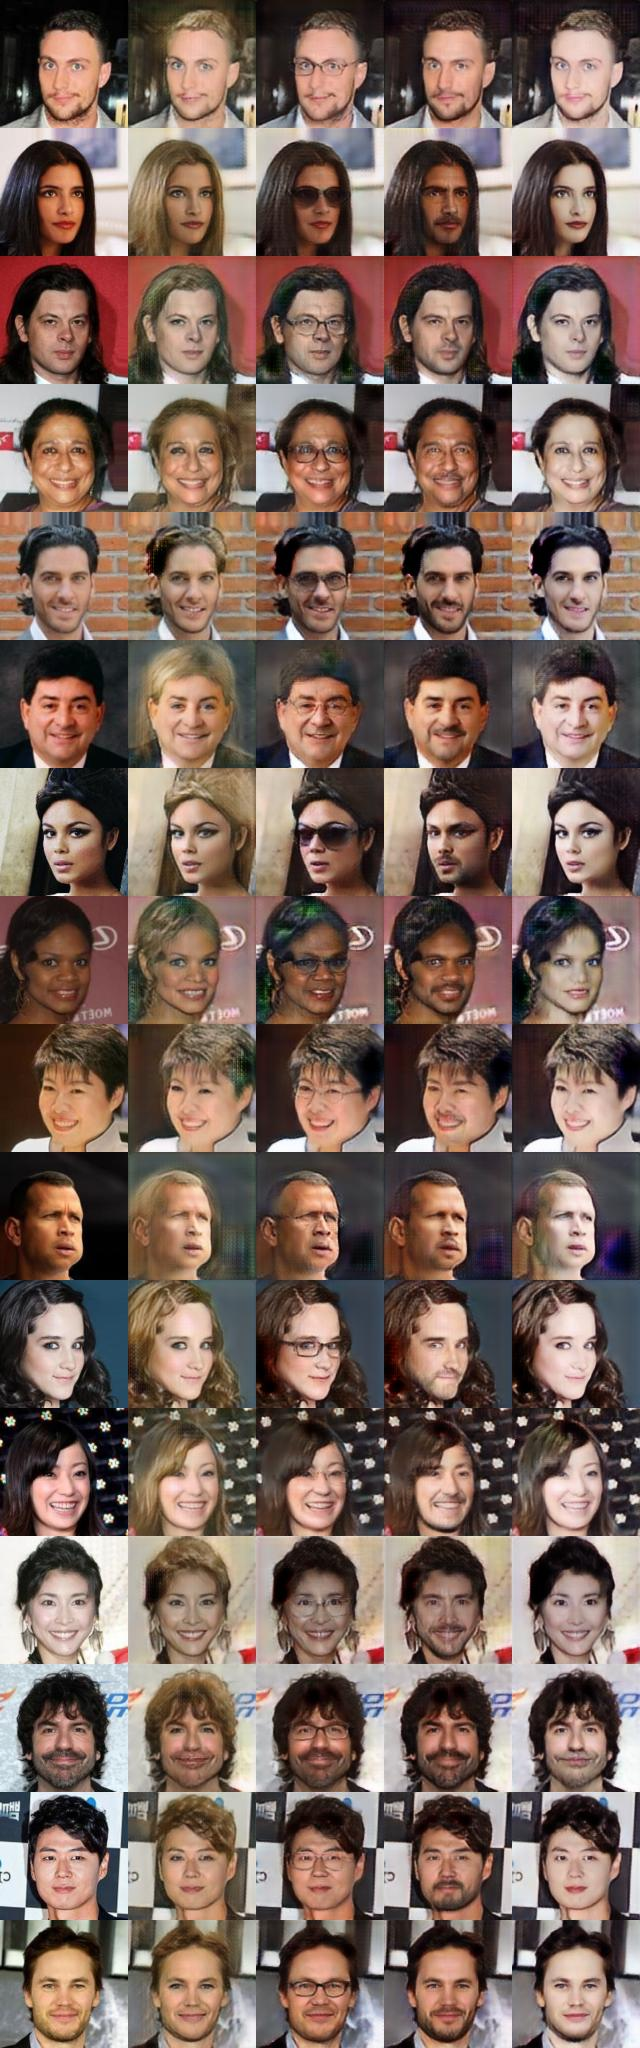
\includegraphics[width=0.49\linewidth,trim={0 59cm 0 0},clip]{figs/mwgan/baseline_050000-images.jpg}
%     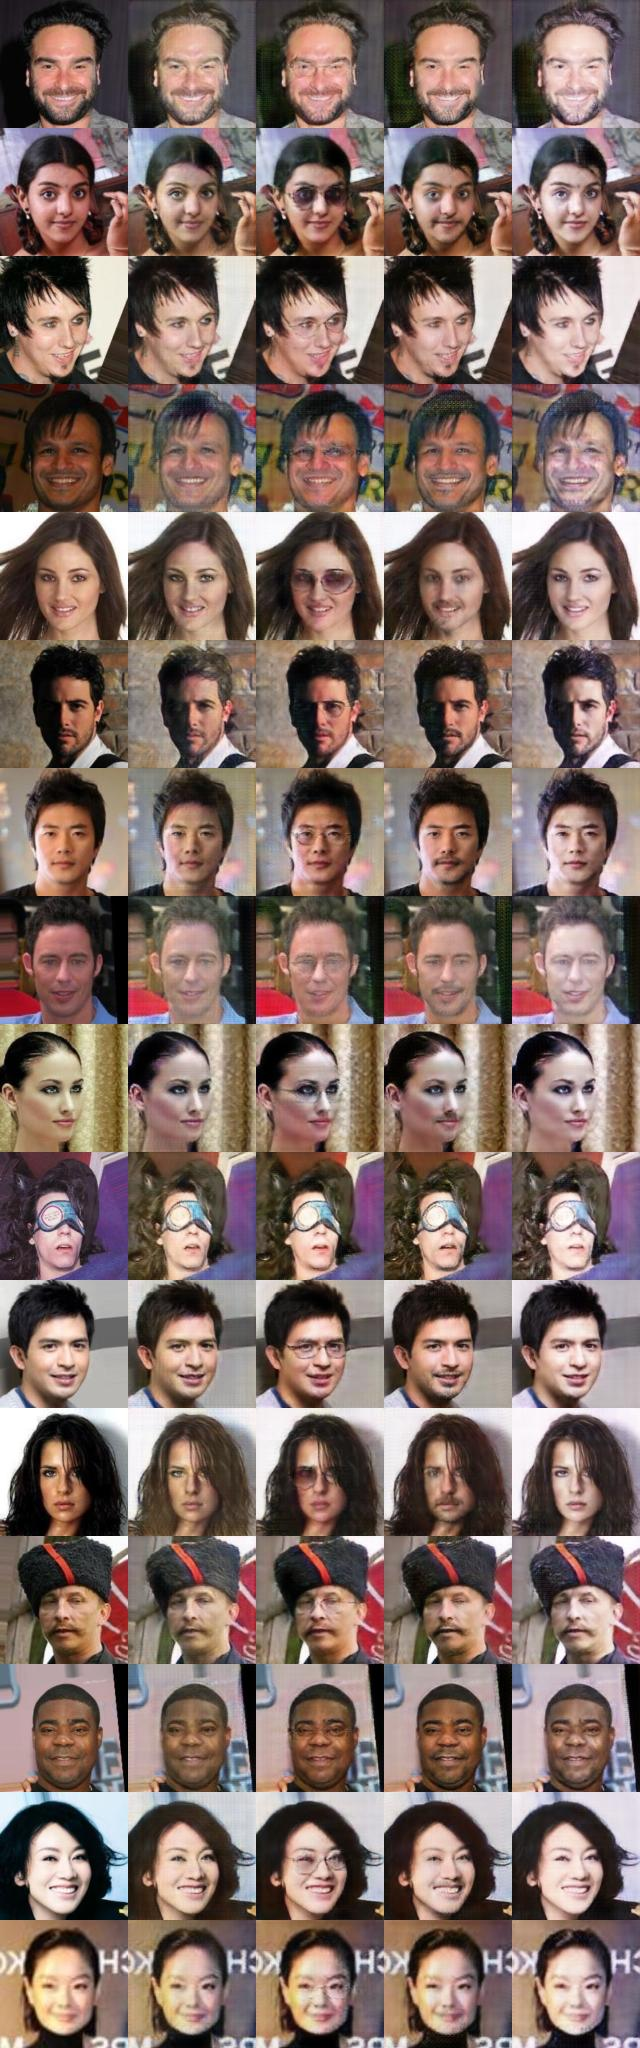
\includegraphics[width=0.49\linewidth,trim={0 58.7cm 0 0},clip]{figs/mwgan/046500-images.jpg}
%     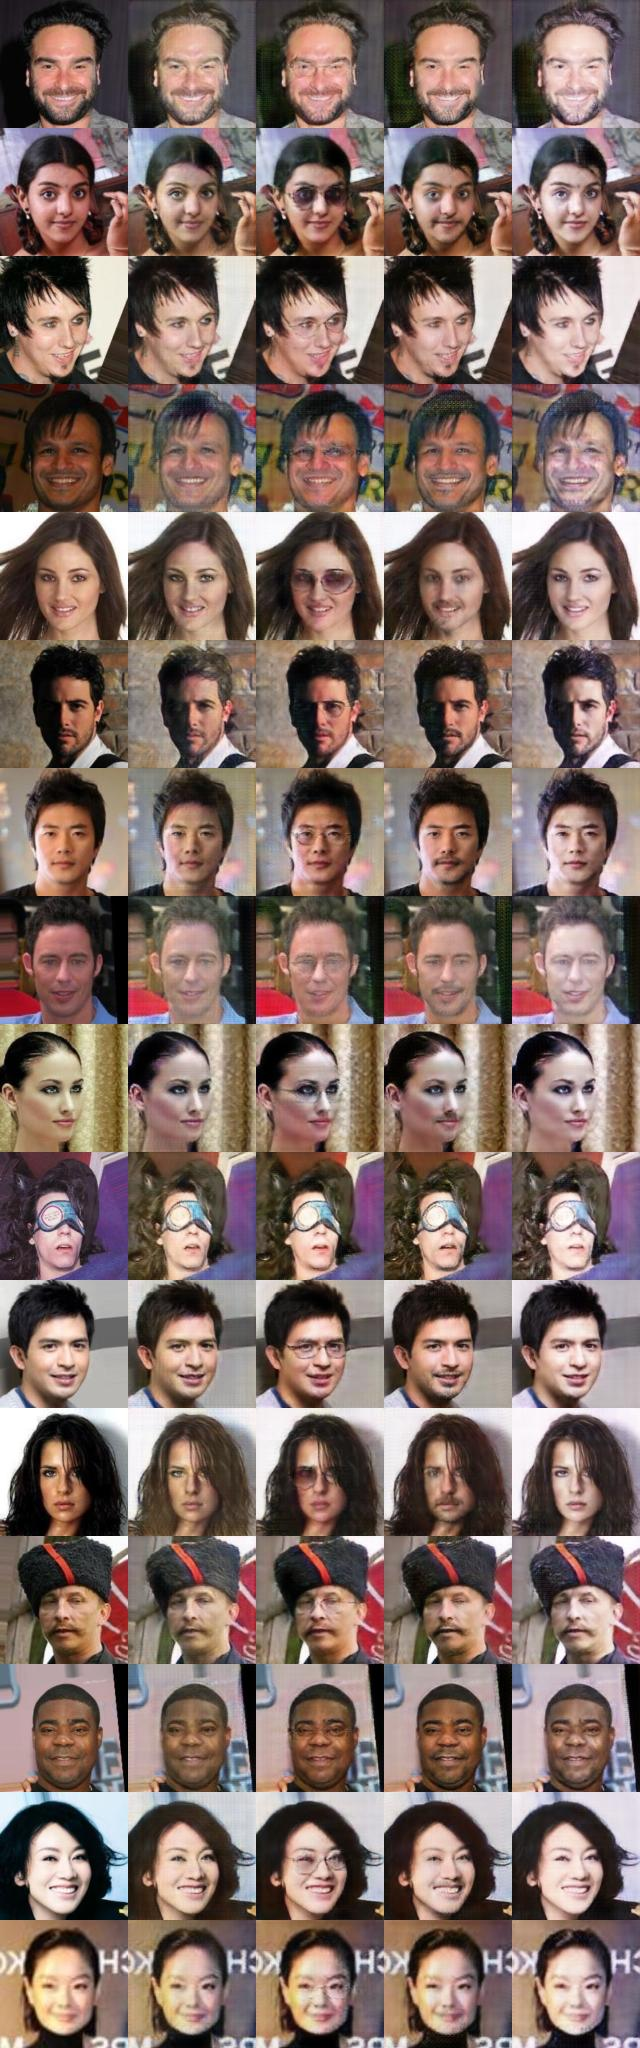
\includegraphics[width=0.49\linewidth,trim={0 0 0 58.7cm},clip]{figs/mwgan/046500-images.jpg}
%     % 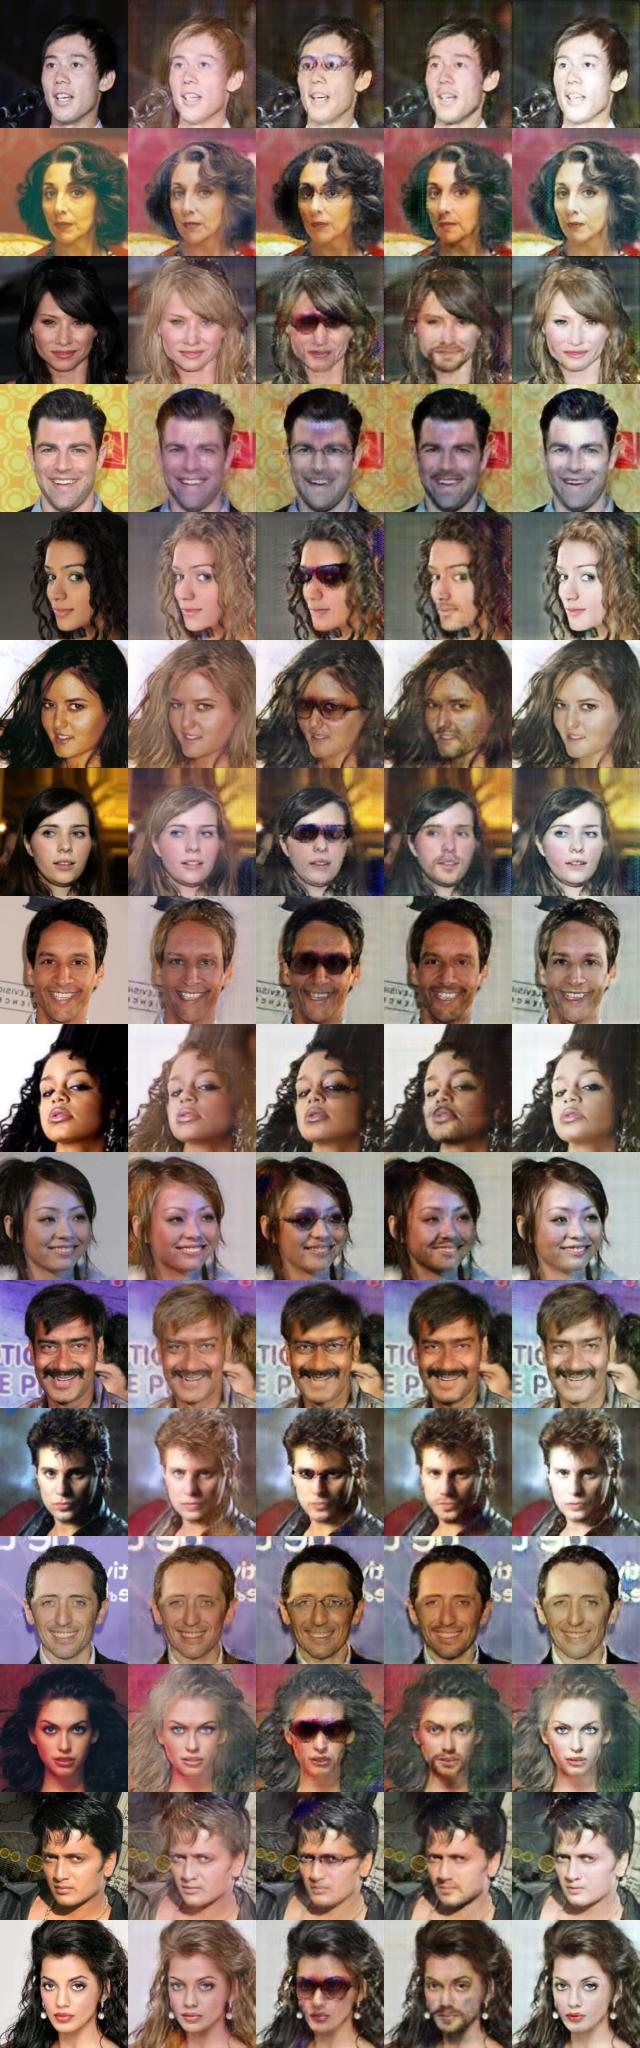
\includegraphics[width=0.49\linewidth,trim={0 63.5cm 0 0},clip]{figs/mwgan/demd_050000-images.jpg}
%     % 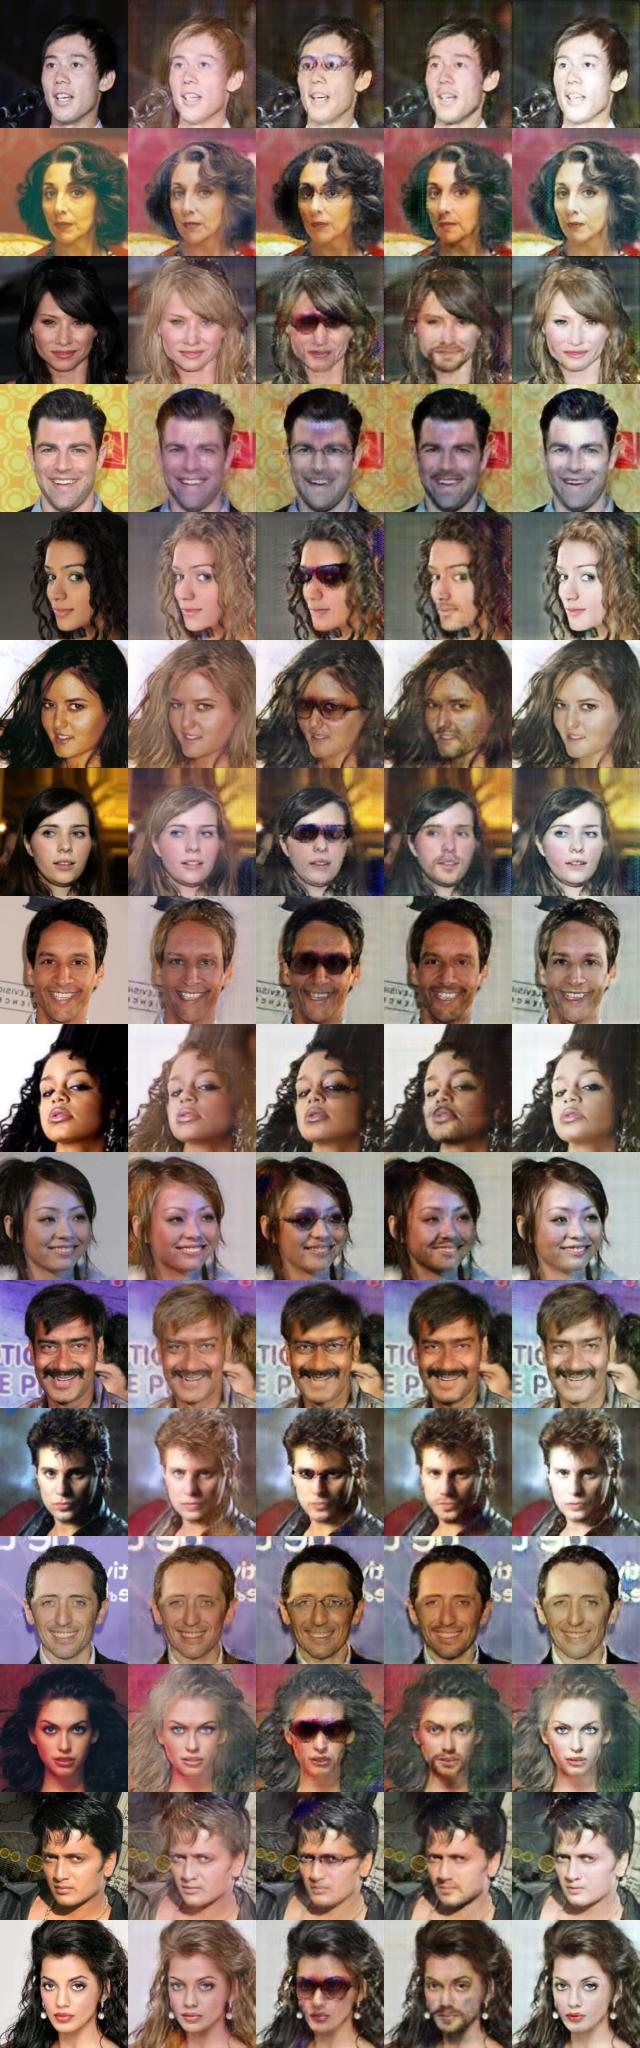
\includegraphics[width=0.49\linewidth,trim={0 63.5cm 0 0},clip]{figs/mwgan/demd_050000-images.jpg}
%     \caption{\footnotesize Six MWGAN+DEMD CelebA image translation results. Each row corresponds to a random sample in the validation set. The leftmost image is the original source image, and sequential columns represent translations to (1) Blonde Hair, (2) Glasses, (3) Mustache, and (4) Pale Skin.\ronak{put labels on top of images? add bar separating original and targets?}}
%     \label{fig:mwgan}
% \end{figure}

\begin{figure*}[t]
    \centering
    \scriptsize
    	Original \quad\; Blond Hair \quad\; Glasses \quad\; Moustache \quad\; Pale Skin \quad\quad Original \quad\; Blond Hair \quad\; Glasses \quad\; Moustache \quad\; Pale Skin \\
    	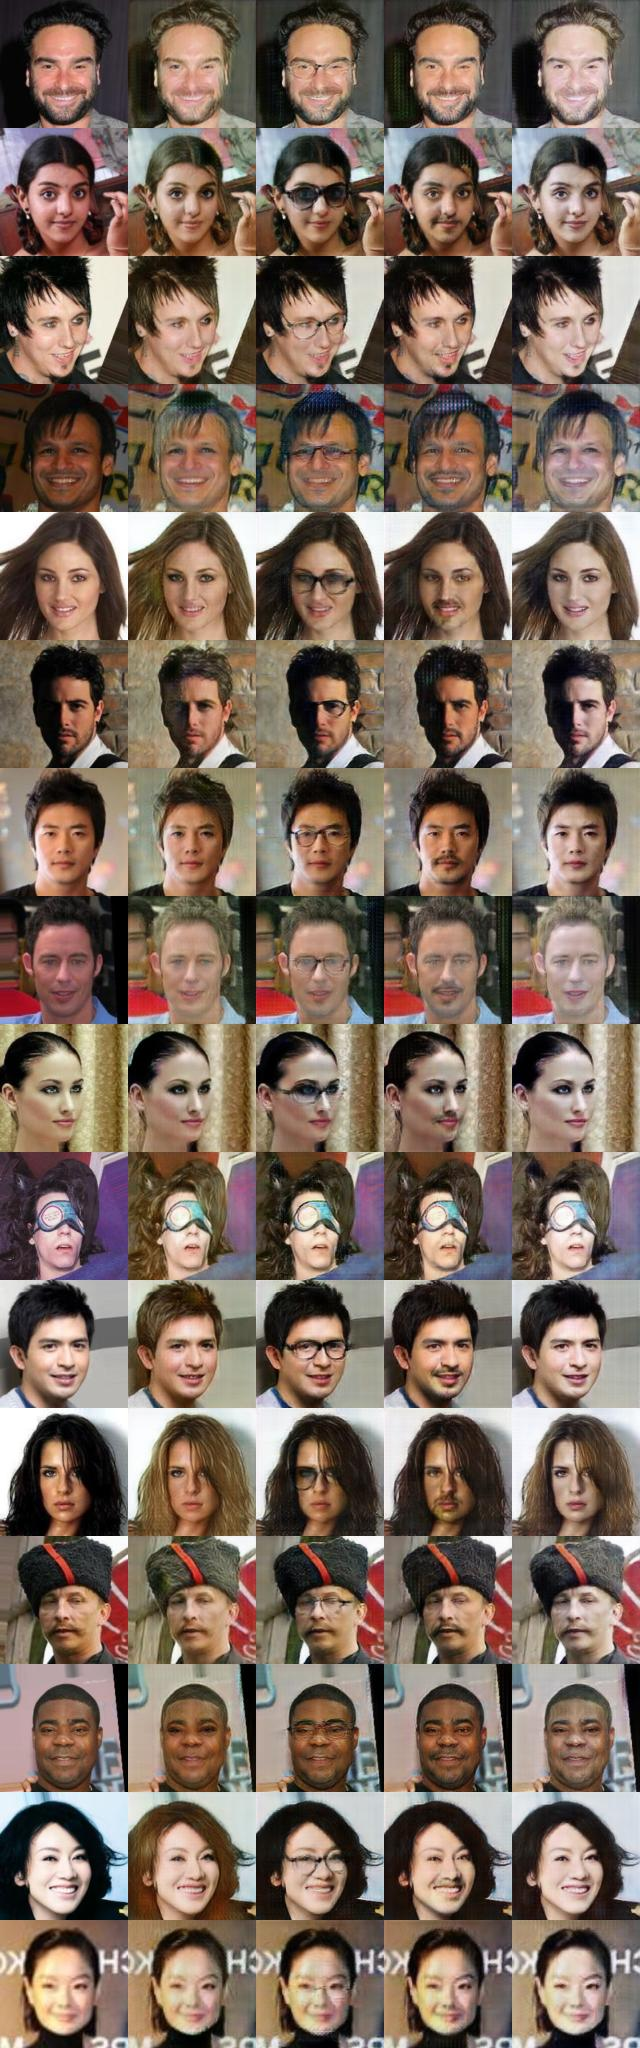
\includegraphics[width=0.49\linewidth,trim={0 58.7cm 0 0},clip]{6_demd/figs/mwgan/069500-images.jpg} 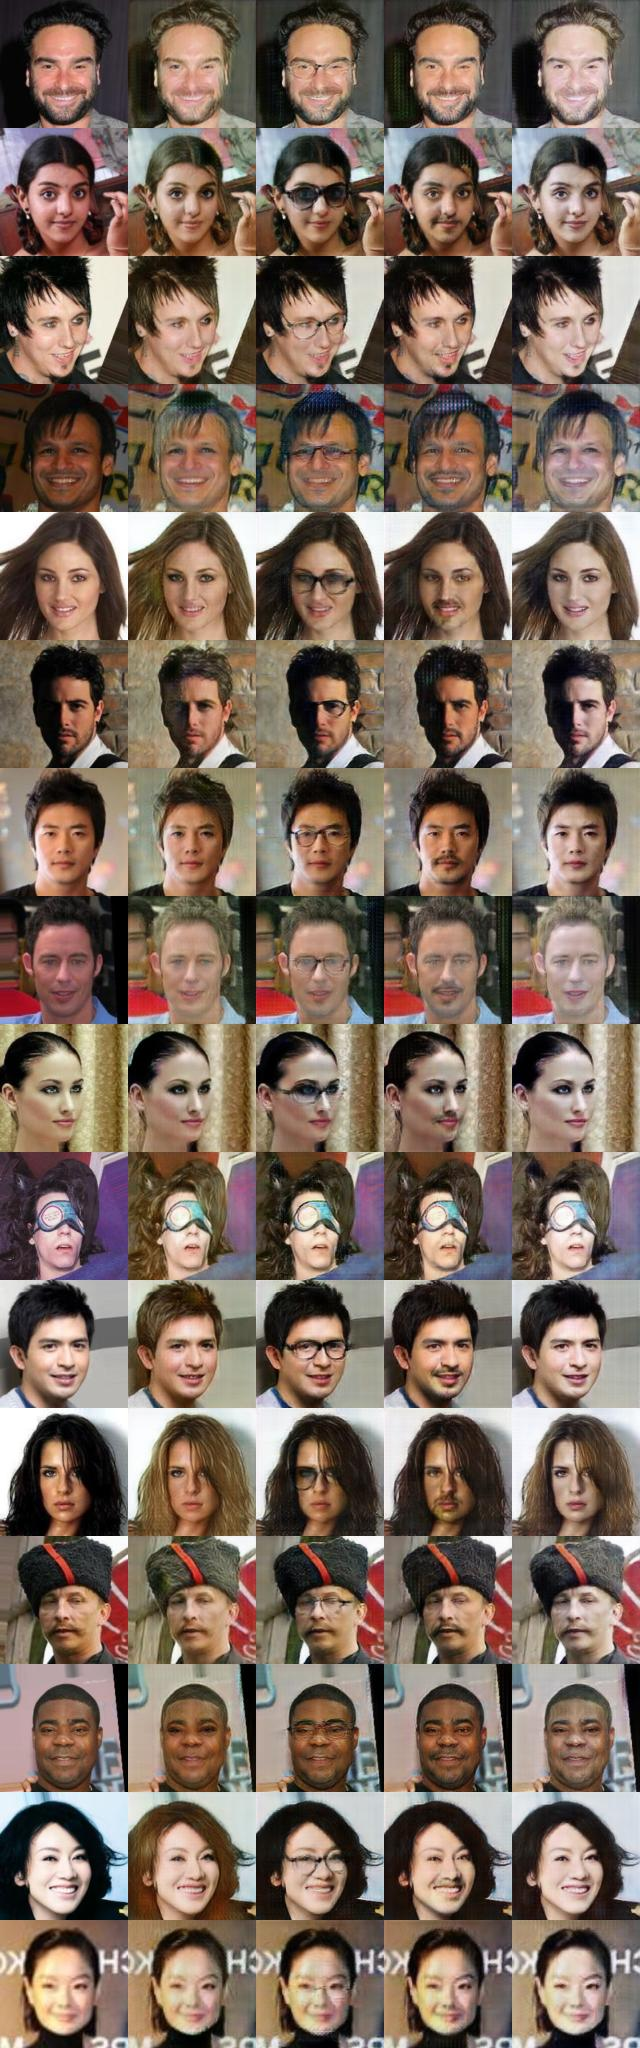
\includegraphics[width=0.49\linewidth,trim={0 0 0 58.7cm},clip]{6_demd/figs/mwgan/069500-images.jpg}
    \caption{Six MWGAN+DEMD CelebA image translation results. Each row corresponds to a random sample in the validation set. The leftmost image is the original source image, and sequential columns represent translations to (1) Blonde Hair, (2) Glasses, (3) Moustache, and (4) Pale Skin. Using DEMD as a relaxation to the Multiple Marginal Matching problem facilitates high quality images translation. For more results see Appendix~\ref{sec:app-mwgan}. }
    \label{fig:mwgan}
\end{figure*}


%%%%%%%%%%%%%%%%%%%%%%% OLD stuff
%%%%%%%%%%%%%%%%%%%%%%% OLD stuff
%%%%%%%%%%%%%%%%%%%%%%% OLD stuff
%%%%%%%%%%%%%%%%%%%%%%% OLD stuff



% \begin{table*}[!t] 
% 	\scriptsize
% 	\setlength\tabcolsep{4pt} % make LaTeX figure out width of inter-column spaces
% 	\caption{\footnotesize Fairness validation results, higher accuracy is better, Lower Fairness measures are better. Higher accuracies \textbf{(ACC)} with lower measures of max Demographic Parity Gap \textbf{(|DP|)},  Equalized Odds Gap \textbf{(|EO|)}, and \textbf{(DEMD)}. \vishnu{Other methods minimize DEMD better than DEMD algorithm itself? Kinda mixed message} \vishnu{Accuracy values should not be in bold. Infact, separate color needs to be used for accuracy column. The idea is that upto 2-4\% drop in accuracy is permissible as long as the fairness measures improve.} \vishnu{Accuracy values are different from this table to the next one! accuracy is kinda redundant information. Best if avoided or moved to the supplement}}
% 	\begin{tabular*}{\linewidth}{l *{3}{c}|*{3}{c}|*{3}{c}|*{3}{c}}
% 		\midrule%\midrule
% 		& \multicolumn{3}{c}{German} & \multicolumn{3}{c}{Adult} & \multicolumn{3}{c}{Crime}& \multicolumn{3}{c}{ACS-Employ} \\
% 		\cmidrule{2-4} \cmidrule{5-7} \cmidrule{8-10} \cmidrule{11-13}
% 		& ACC & |DP| & |EO| & DEMD & ACC  & |DP| & |EO| & DEMD & ACC & |DP| & |EO| & DEMD & ACC & |DP| & |EO| & DEMD \\ 
% 		\midrule
% 		None & 0.180 & 0.134 & 1.694 & 0.382 & 0.446 & 2.858 & 0.351 & 0.306 & 3.556 & 0.365 & 0.251 & 4.778 \\
% DP-Reg. & 0.169 & 0.128 & 1.600 & 0.383 & 0.446 & 2.832 & 0.362 & 0.250 & 3.705 & 0.477 & 0.276 & 5.024 \\
% EO-Reg. & 0.143 & 0.116 & 1.425 & 0.377 & 0.442 & 2.830 & 0.363 & 0.311 & 3.055 & 0.377 & 0.256 & 4.818 \\
% Bary & 0.177 & 0.134 & 1.645 & 0.362 & 0.442 & 2.811 & 0.377 & 0.256 & 2.726 & 0.571 & 0.497 & 4.376 \\
% DEMD & 0.145 & 0.117 & 1.443 & 0.364 & 0.438 & 2.688 & 0.288 & 0.361 & 3.101 & 0.334 & 0.236 & 3.598 \\
% % 		None & 0.77 & 0.17 & 0.11 & 1.69 & \textbf{0.84} & 0.18 & 0.13 & 1.69 & \textbf{0.84} & 0.38 & 0.45 & 2.86 & \textbf{0.80} & 0.35 & 0.31 & 3.56 \\
% % DP-Reg. & 0.77 & 0.16 & 0.10 & 1.50 & \textbf{0.84} & 0.17 & 0.13 & 1.60 & 0.83 & 0.37 & 0.44 & 2.65 & 0.79 & 0.36 & \textbf{0.25} & 3.71 \\
% % EO-Reg. & 0.75 & 0.20 & 0.11 & 1.59 & \textbf{0.84} & 0.14 & \textbf{0.12} & 1.43 & 0.83 & \textbf{0.35} & \textbf{0.43} & 2.54 & 0.79 & 0.53 & 0.36 & 3.06 \\
% % Bary & \textbf{0.79} & 0.27 & 0.17 & 1.50 & 0.81 & \textbf{0.13} & 0.14 & \textbf{0.99} & 0.81 & \textbf{0.35} & 0.44 & \textbf{2.61} & 0.79 & 0.38 & 0.26 & \textbf{2.73} \\
% % DEMD & 0.77 & \textbf{0.14} & \textbf{0.09} & \textbf{1.41} & \textbf{0.84} & 0.15 & \textbf{0.12} & 1.44 & 0.83 & 0.36 & 0.44 & 2.69 & \textbf{0.80} & \textbf{0.29} & 0.36 & 3.10 \\
% % 		None & XXYY & XXYY & XXYY & XXYY  & XXYY & XXYY & XXYY & XXYY & XXYY & XXYY & XXYY & XXYY & XXYY & XXYY & XXYY & XXYY \\
% % 		DP & XXYY & XXYY & XXYY & XXYY & XXYY & XXYY & XXYY & XXYY & XXYY & XXYY & XXYY & XXYY & XXYY & XXYY & XXYY & XXYY \\
% % 		EO & XXYY & XXYY & XXYY & XXYY & XXYY & XXYY & XXYY & XXYY & XXYY & XXYY & XXYY & XXYY & XXYY & XXYY & XXYY & XXYY \\
% % 		Bary & XXYY & XXYY & XXYY & XXYY & XXYY & XXYY & XXYY & XXYY & XXYY & XXYY & XXYY & XXYY & XXYY & XXYY & XXYY & XXYY \\
% % 		DEMD & XXYY & XXYY & XXYY & XXYY & XXYY & XXYY & XXYY & XXYY & XXYY & XXYY & XXYY & XXYY & XXYY & XXYY & XXYY & XXYY \\
% 		\midrule%\midrule
% 	\end{tabular*}
% 	\label{tab:fair_results}
% \end{table*} 

% \begin{table}[]
%     \centering
%     \begin{tabular}{c|cccc}
%         \toprule
%         $\lambda_{reg}$ & Acc & DP Gap & EO Gap & EMD \\
%         \midrule
%         0.00 & 0.776 & 0.665 & 0.723 & 3.352 \\
%         0.01 & 0.776 & 0.670 & 0.726 & 3.050 \\
%         0.02 & 0.776 & 0.474 & 0.527 & 2.317 \\
%         0.03 & 0.773 & 0.485 & 0.531 & 1.965 \\
%         0.04 & 0.763 & 0.506 & 0.540 & 1.575 \\
%         0.05 & 0.738 & 0.339 & 0.356 & 1.149 \\
%         0.06 & 0.670 & 0.178 & 0.200 & 0.662 \\
%         0.07 & 0.594 & 0.006 & 0.005 & 0.372 \\
%         0.08 & 0.590 & 0.000 & 0.000 & 0.031 \\
%         0.09 & 0.590 & 0.000 & 0.000 & 0.000 \\
%         0.10 & 0.590 & 0.000 & 0.000 & 0.000 \\\bottomrule
%     \end{tabular}
%     \caption{Outcome measures as a function of regularization parameter when our EMD regularizer is used.}
%     \label{tab:reg_sweep}
% \end{table}

% \begin{figure}
%     \centering
%     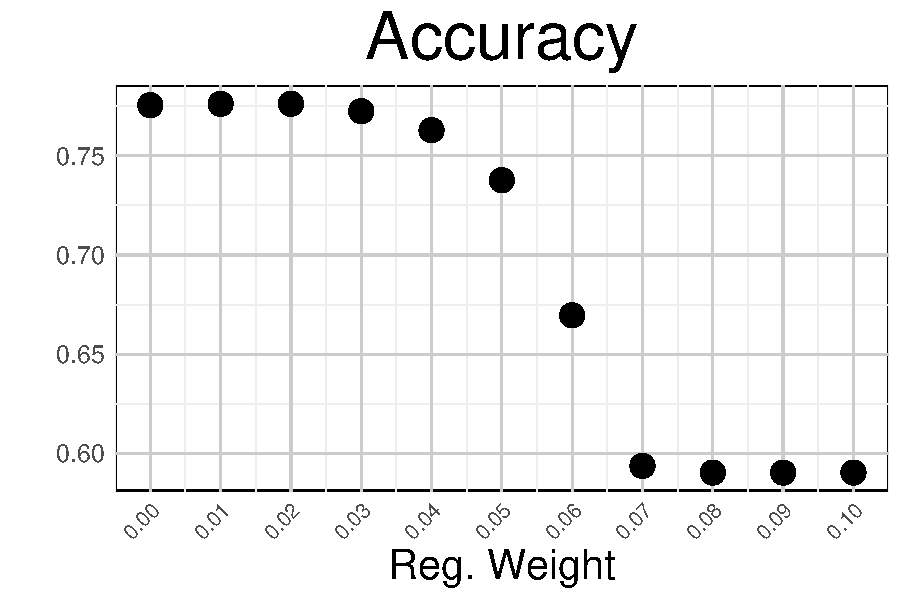
\includegraphics[width=0.24\columnwidth]{figs/regweights/lambdas_Acc.pdf}
%     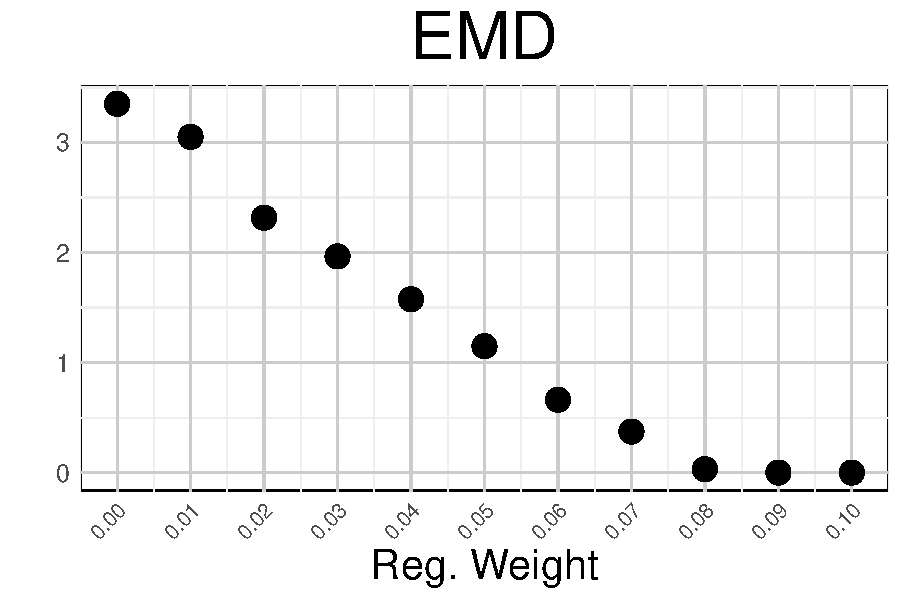
\includegraphics[width=0.24\columnwidth]{figs/regweights/lambdas_DEMD.pdf}
%     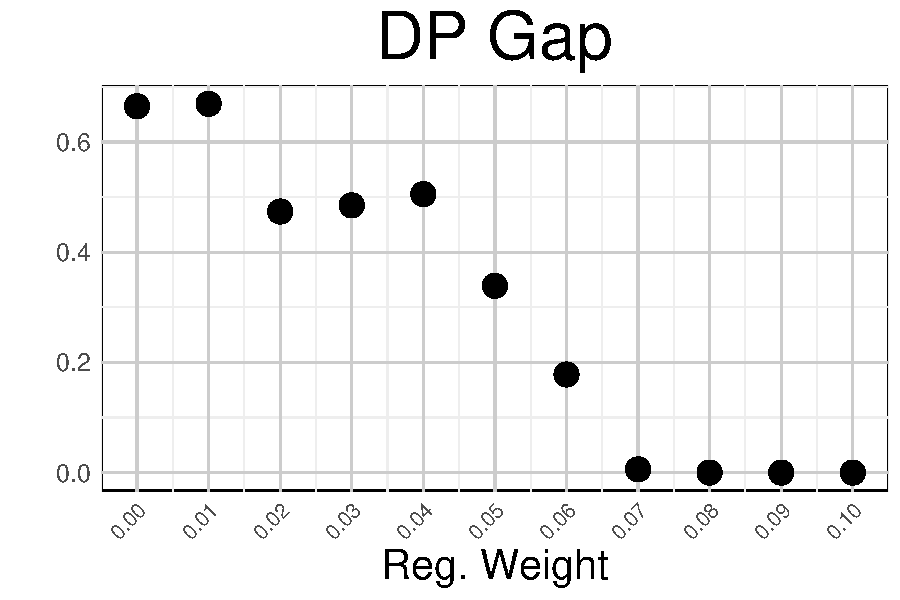
\includegraphics[width=0.24\columnwidth]{figs/regweights/lambdas_DPgap.pdf}
%     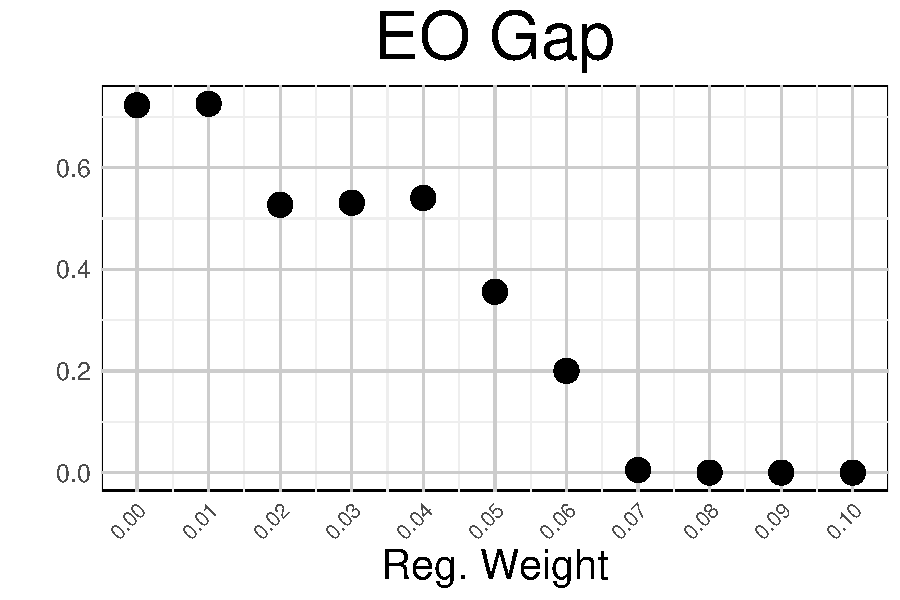
\includegraphics[width=0.24\columnwidth]{figs/regweights/lambdas_EOgap.pdf}
%     \caption{Outcome measures as a function of regularization parameter when our EMD regularizer is used. Output measures of fairness track the upstream EMD constraint, and follow the same accuracy-fairness tradeoff.}
%     \label{fig:reg_sweep}
% \end{figure}

% \begin{table*}[ht]
%     \centering\small
%     \begin{tabular}{llcccccc}
%     \toprule
%         RegType & $\lambda_{reg}$ & Total Acc & MinAcc & MaxAcc & $|DP_{max} - DP_{min}|$ & $|EO_{max} - EO_{min}|$ & D-EMD \\
%         \midrule
%         Log. Reg. & 0.0   & 0.786 & 0.699 & 0.867 & 0.474 & 0.522 & 3.331 \\
%                   & 0.001 & 0.786 & 0.708 & 0.878 & 0.481 & 0.526 & 3.332 \\
%                   & 0.01  & 0.590 & 0.200 & 0.878 & 0.000 & 0.000 & 0.044 \vspace{0.1in}\\
                  
%         2NN       & 0.0   & 0.795 & 0.600 & 0.856 & 0.371 & 0.327 & 3.265 \\
%                   & 0.001 & 0.794 & 0.600 & 0.878 & 0.354 & 0.335 & 2.976 \\
%                   & 0.01  & 0.648 & 0.200 & 0.878 & 0.108 & 0.100 & 0.062 \\
% \bottomrule\\
%     \end{tabular}
%     \caption{Validation results for various models and regularization weights on the ACS Income prediction task including demographic parity
% (DP) and equality of opportunity (EO) spreads. }
%     \label{tab:acsinc}
% \end{table*}


% \begin{table*}[ht]
%     \centering\small
%     \begin{tabular}{llcccccc}
%     \toprule
%         Model & $\lambda_{reg}$ & Total Acc & MinAcc & MaxAcc & $|DP_{max} - DP_{min}|$ & $|EO_{max} - EO_{min}|$ & D-EMD \\
%         \midrule
%         Log. Reg. & 0.0   & 0.786 & 0.699 & 0.867 & 0.474 & 0.522 & 3.331 \\
%                   & 0.001 & 0.786 & 0.708 & 0.878 & 0.481 & 0.526 & 3.332 \\
%                   & 0.01  & 0.590 & 0.200 & 0.878 & 0.000 & 0.000 & 0.044 \vspace{0.1in}\\
                  
%         2NN       & 0.0   & 0.795 & 0.600 & 0.856 & 0.371 & 0.327 & 3.265 \\
%                   & 0.001 & 0.794 & 0.600 & 0.878 & 0.354 & 0.335 & 2.976 \\
%                   & 0.01  & 0.648 & 0.200 & 0.878 & 0.108 & 0.100 & 0.062 \\
% \bottomrule\\
%     \end{tabular}
%     \caption{Validation results for various models and regularization weights on the ACS Income prediction task including demographic parity
% (DP) and equality of opportunity (EO) spreads. }
%     \label{tab:acsinc}
% \end{table*}

% \begin{table*}[ht]
%     \centering\small
%     \begin{tabular}{llcccccc}
%     \toprule
%         Model & $\lambda_{reg}$ & Total Acc & MinAcc & MaxAcc & $|DP_{max} - DP_{min}|$ & $|EO_{max} - EO_{min}|$ & D-EMD \\
%         \midrule
%         Log. Reg.  & 0.0  & 0.769 & 0.500 & 0.824 & 0.194 & 0.194 & 2.200  \\
%                   & 0.01 & 0.769 & 0.500 & 0.824 & 0.194 & 0.185 & 2.124  \\
%                   & 0.1  & 0.546 & 0.500 & 0.632 & 0.000 & 0.000 & 0.093  \vspace{0.1in}\\
%         2NN        & 0.0 & 0.806 & 0.744 & 1.000 & 0.167 & 0.176 & 2.844  \\
%                   & 0.01 & 0.806 & 0.774 & 1.000 & 0.165 & 0.180 & 2.644  \\
%                   & 0.1 & 0.645 & 0.500 & 0.708 & 0.244 & 0.203 & 0.059  \\
% \bottomrule\\
%     \end{tabular}
%     \caption{Validation results for various models and regularization weights on the ACS Employment prediction task including demographic parity
% (DP) and equality of opportunity (EO) spreads.}
%     \label{tab:acsemp}
% \end{table*}
\section{Conclusion}
Our selection scheme identifies a subset of parameters to update and significantly reduces compute requirements for standard Hessian unlearning. 
%For unlearning, While retraining of small models is a possibility, but unavailability of full training set and for larger models, unlearning is desired.
For smaller networks with a large number of removals, retraining may be effective, but when full training sets are not available or retraining is costly, unlearning in some form is needed. 
We show the ability to approximately unlearn for large models prevalent in vision, a capability that has not so far been demonstrated.  

%\paragraph{Social Impact.} 
%This work 
%is motivated by social considerations of 
%modern ML/Vision models. 
%Indiscriminate use of personal data in training 
%large AI models is ethically questionable 
%and sometimes illegal. We need mechanisms to ensure that AI models operate 
%within boundaries specified by society 
%and legal guardrails. As opt-out laws get 
%implemented, compliance on the service-provider end will entail costs. 
%While our contributions cannot guarantee perfect forgetting, with additional 
%validation they can become a part of a suite of methods for unlearning. 

% \section*{Acknowledgements}
% This work was supported by funding su